\documentclass[conference]{IEEEtran}
\IEEEoverridecommandlockouts
\usepackage{cite}
\usepackage{amsmath,amssymb,amsfonts}
\usepackage{algorithmic}
\usepackage{graphicx}
\usepackage{textcomp}
\usepackage{xcolor}


\usepackage{listings}
\usepackage{xcolor}

\usepackage{tabularx}
\usepackage{booktabs}

\lstset{
  basicstyle=\ttfamily\small,
  frame=single,
  backgroundcolor=\color{gray!5},
  breaklines=true,
}

\def\BibTeX{{\rm B\kern-.05em{\sc i\kern-.025em b}\kern-.08em
    T\kern-.1667em\lower.7ex\hbox{E}\kern-.125emX}}

\begin{document}

\title{From PDF to Knowledge graph: A Fine-tuned LLM vs RAG-KG vs Zero-shot LLM comparison \\
{\footnotesize Natural Language Processing and Text Mining - Project 24} \\
{\small \textbf{Code available at:} \texttt{https://github.com/raphsa/pdf\_to\_KnowledgeGraph\_LLM}}
}

\author{\IEEEauthorblockN{Raffaele Sali}
\IEEEauthorblockA{rsali25@student.oulu.fi}
\and
\IEEEauthorblockN{Martina Vianello}
\IEEEauthorblockA{mvianell25@student.oulu.fi}
\and
\IEEEauthorblockN{Beatrice Zani}
\IEEEauthorblockA{bzani25@student.oulu.fi}
}

\maketitle

\begin{abstract}
This project presents a modular pipeline that transforms complex, domain-specific documents into structured, queryable knowledge for grounded language model applications. The workflow begins with PDF ingestion and parsing, extracting text and tables with section-level metadata. A domain ontology defines key entities and relations in food, nutrition, and health, guiding entity recognition and relation extraction to generate validated triples. These are stored in a knowledge graph, enabling structured exploration and fact retrieval. From this graph, a grounded instruction–response dataset is automatically generated, supporting fine-tuning and evaluation of large language models. The system includes Zero-shot, RAG-KG, and fine-tuned baselines, evaluated for factuality, faithfulness, and hallucination control. Finally, a Gradio demo illustrates real-time question answering with source-grounded explanations. The framework demonstrates a scalable approach to integrating structured semantic knowledge with interpretable language model reasoning.
\end{abstract}

\begin{IEEEkeywords}
Knowledge Graph, NLP, LLM, RAG-KG, Text Mining, Fine-Tuning
\end{IEEEkeywords}

% Include sections
\section{Introduction}
Knowledge representation in structured form has become an increasingly important pillar in the development of intelligent systems. A key paradigm is the Knowledge Graph (KG), which represents real-world entities as nodes and the relationships between them as edges, enabling both human-readable and machine-processable semantics. Parallel to this, the advent of large language models (LLMs) has transformed how unstructured textual data is used and processed. However, while LLMs excel at language understanding, they are prone to producing content that is not grounded in factual evidence or reliable structure, commonly termed \textit{hallucinations}. Integrating knowledge graphs with LLMs can help ground their outputs in structured knowledge and reduce unanchored generation.
Documents in PDF format remain one of the most common mediums in many domains (academic, technical, regulatory). Yet, extracting structured knowledge from PDFs poses substantial technical challenges: the text may be unstructured, include tables and figures, hierarchical headings, and embedded images.

In this context, our project addresses the following research problem: how to extract structured knowledge from a domain-specific PDF (in the food domain), construct a knowledge graph (KG), and use that graph to generate grounded instruction-response pairs in order to fine-tune an LLM, and then compare this fine-tuned model with two baselines: (i) zero-shot LLM, and (ii) retrieval-augmented generation over the KG (RAG-KG). 

Recent dietary guidelines such as the Finnish “National Nutrition Recommendations 2024” emphasise not only individual health, but also the planetary health consequences of food production and consumption. For instance, food consumption in Finland has been estimated to account for around $20 \%$ of the annual climate impacts of the average consumer, and diets aligned with nutritional and sustainability goals can potentially reduce the climate footprint by over one-third. These guidelines are produced through large-scale surveys, modelling of consumption patterns, and systematic reviews of nutritional and environmental research.
As the main source of domain knowledge, this project relies on the “Sustainable Health from Food – National Nutrition Recommendations 2024” report by the Finnish Institute for Health and Welfare \cite{thl2024nutrition}. This document provides an evidence-based synthesis of food and health recommendations, yet it exists primarily as a human-readable PDF, where valuable knowledge is distributed across sections, tables, and figures.
In this project, we take this complex PDF as our source document and convert its contents into structured knowledge within the food and nutrition domain. By doing so, we establish a pipeline that enables downstream tasks—such as fact-based instruction–response generation and fine-tuning of large language models—and allow for systematic comparison between grounded and ungrounded model settings.



\section{Methodology}

% add description about this section what it contains and what it's going to explain

The methodology of this project follows a modular pipeline designed to extract structured knowledge from a complex, domain-specific document and to use it for large language model (LLM) fine-tuning and evaluation.
The methodology is organised into several components, each corresponding to one stage of the pipeline:
\begin{itemize}
\item PDF ingestion and parsing;
\item Domain ontology and ontology draft;
\item NER and keyphrase extraction;
\item Relation extraction and triple building;
\item Knowledge graph construction and storage;
\item Instruction-response dataset creation (grounded);
\item Fine-tuning setup;
\item Evaluation (Quality, Factuality, Faithfulness);
\item Hallucination detection and mitigation;
\item Delivery and demo.
\end{itemize}
This section describes each component in detail.

\subsection{PDF ingestion and parsing}

The PDF ingestion and parsing system was designed to convert a complex, structured PDF document into a machine-readable format suitable for data analysis and information retrieval. The process integrates several Python libraries to detect, extract, and organise both textual and tabular information while preserving the logical structure of the original document.
The first stage focuses on identifying and parsing the table of contents (\texttt{TOC}), in order to then get a better division for text chunks. Using \texttt{PyMuPDF}, the entire PDF and the section titled “Contents” or “Table of Contents” is scanned. This section is then cleaned of irrelevant page artefacts such as publisher names or header text. After finding the section, through the use of regular expressions, each line of the \texttt{TOC} is decomposed into a section title and a corresponding page number. The resulting output is normalized and assembled into a tabular form using \texttt{pandas}, which produces a structured index of section titles and their starting pages. This index forms the backbone of the document’s hierarchical reconstruction.

In the second stage, the program iteratively traverses the full text of the PDF, page by page, to associate each segment of text with its correct section heading. Each page is read as a series of lines, and pattern matching is used to identify when a new section begins, based on the \texttt{TOC} entries detected earlier. Text that falls between these headings is aggregated and labelled as belonging to that specific section. 
The final result is a set of text chunks in which every passage is linked to a document section and page number. These are stored in a JSON Lines (\texttt{.jsonl}) file to facilitate subsequent analysis and/or indexing.

\begin{figure}[h!]
\centering
\begin{lstlisting}
{"page": 33, "section": "Carbohydrates and fibre", "text": "The recommended intake of carbohydrates is 45 to 60% of the total daily energy intake (E%). The recommended intake..."}
{"page": 33, "section": "Fat", "text": "The recommendations for fat intake emphasise quality, that is, the fatty acid composition of the diet. The recommended fat intake is 25 to 40% of the total daily energy intake (E%). An inadequate fat intake.."}
\end{lstlisting}
\caption{Example of parsed text output in JSONL format.}
\label{fig:jsonl_example}
\end{figure}


Parallel to text extraction, a third process handles table recognition. The script employs \texttt{Camelot} in two configurations, \texttt{STREAM} and \texttt{LATTICE}, to capture both text-aligned and line-bordered tables.
Every detected table is cleaned, converted into a \texttt{pandas DataFrame}, and exported as a \texttt{CSV} file, together with metadata indicating the page number, table dimensions, and file path. In this way, textual and tabular data are separated but remain referentially linked to the same document structure.
Together, these steps produce a structured dataset from the original PDF: a machine-readable representation of both the narrative and the quantitative content of the report. This enables further computational analysis, such as keyword extraction or thematic clustering.



\subsection{Domain schema and ontology draft}

To enable structured representation of entities and relations extracted from the source document, a domain-specific ontology was designed for the food, nutrition, and health domain. The ontology defines the conceptual schema for the knowledge graph and provides standardized classes, attributes, and relations linking ingredients, nutrients, dietary guidelines, techniques, health outcomes and environmental impacts.

The ontology was implemented in \texttt{YAML} format and assigned a base URI (\texttt{http://example.org/food\#}) for semantic consistency. It serves as a lightweight conceptual model aligning with RDF principles, enabling conversion to \texttt{Turtle (TTL)} or \texttt{RDF/XML} for graph storage and querying.

Six main classes were defined:
\begin{itemize}
    \item \textbf{ingredient} – physical food items or raw materials (e.g., wheat, fish, legumes) with attributes for group, origin, and environmental impact.
    \item \textbf{nutrient} – chemical or biological components contributing to physiological functions (e.g., protein, vitamin C, omega-3).
    \item \textbf{technique} – preparation or processing methods influencing food properties, safety, or nutrient content (e.g., boiling, fermentation).
    \item \textbf{dietaryGuideline} – official recommendations specifying consumption or preparation guidance for health and sustainability goals.
    \item \textbf{healthOutcome} – measurable health effects or conditions linked to nutrients or dietary behaviors (e.g., cardiovascular risk, bone health).
    \item \textbf{environmentImpact} – quantified environmental effects associated with foods or production processes (e.g., greenhouse gas emissions, water use).
\end{itemize}

The ontology also defines key relations connecting these entities, such as:
\begin{itemize}
    \item \textbf{hasNutrient}: ingredient $\rightarrow$ nutrient.
    \item \textbf{usesTechnique}: ingredient $\rightarrow$ technique.
    \item \textbf{hasGuideline}: ingredient $\rightarrow$ dietaryGuideline
    \item \textbf{aimsToImprove}: dietaryGuideline $\rightarrow$ healthOutcome
    \item \textbf{hasEnvironmentalImpact}: ingredient $\rightarrow$ environmentImpact
    \item \textbf{affectsRiskOf}: nutrient $\rightarrow$ healthOutcome
\end{itemize}

Each relation includes domain, range, and cardinality constraints to ensure schema consistency during triple generation.

The ontology acts as a unifying layer between raw textual information and the structured knowledge graph. It ensures that all extracted entities and relations adhere to consistent categories and relation types. The design intentionally balances minimalism (for computational efficiency) and expressivity (for coverage of nutritional, environmental, and health dimensions).


\subsection{NER and keyphrase extraction}
The named entity recognition (NER) and keyphrase extraction stage focused on identifying and normalizing domain-specific entities mentioned in the text. This process aimed at generating a structured list of unique entities, aligned with the previously defined ontology, to create the base of the knowledge graph population. 

Firstly, a seed vocabulary was created to list an initial set of example entities extracted from the parsed text. Each text chunk was analyzed and cleaned (for instance, by removing punctuation), then occurrences of ontology classes were detected by using predefined keyword lists and regular expressions. Only the terms appearing in at least two distinct chunks were kept. The resulting list of seeds was then cleaned and refined by removing irrelevant terms and adding missing but semantically important ones. An example of terms saved for the class \textbf{ingredient} includes: “alcohol”, “barley”, “beans”, “berries”, “butter”, “cereals”, “cheese”.

The second step consisted in generating the final entities file, where each line contains information about a unique entity found in the extracted text. This process combined the raw text, the seeds created earlier and the ontology to perform entity recognition and normalization. Using \texttt{spaCy}, the algorithm scanned the text chunks looking for mentions of the seed examples, then grouped synonyms and merged aliases. For each merged group, the most generic label was selected as the canonical entity name and a unique identified was assigned. The most important fields stored for each unique mention are:
\begin{itemize}
    \item\textbf{id} - unique identifier created from the ontology class prefix and an incremental index.
    \item \textbf{type} - ontology class associated with the entity.
    \item \textbf{label} - canonical name of the entity.
    \item \textbf{mentions} - list of mentions of the entity found in the text, each including page reference and context.
\end{itemize}

After this NER pipeline, the resulting file, saved in JSON Lines (\texttt{.jsonl}) format, provided the starting point for the next steps of execution such as relation extraction and triple building.

\begin{figure}[h!]
\centering
\scriptsize
\begin{lstlisting}[
    columns=fullflexible, % Allows characters to be spaced flexibly
    breaklines=true,      % Tells LaTeX to wrap long lines
    breakatwhitespace=true, % Break only at whitespace (good for code readability)
    basicstyle=\scriptsize\ttfamily, % Ensures the style is set
    frame=single % If you have a frame, this might help control it
]
{"id": "http://example.org/food#ingredient_salt", "type": "ingredient", "label": "salt", "mentions": [{"page": 5, "section": "Preface", "text_span": [556, 560], "context": "... challenges that remain are excessive salt and saturated fat intakes and insufficient fibre intake."}, {"page": 5, "section": "Preface", "text_span": [931, 935], "context": "... vegetable oils, fish and nuts, and limit the use of salt."}]}
\end{lstlisting}
\caption{Example of entity in JSONL format.}
\label{fig:entity_example}
\end{figure}

\subsection{Relation extraction and triple building}
Following entity extraction, a rule-based system was implemented to construct a semantic representation of the document in the form of an RDF knowledge graph. This stage transforms the previously identified entities, such as ingredients, nutrients, techniques, or health outcomes, into formally defined relationships, enabling structured querying and reasoning.
The process begins by reading the JSONL file containing the detected entities and all their textual mentions. Each record includes the entity’s label, its ontology type (e.g., ingredient, nutrient, healthOutcome), and metadata describing where it appears in the document, such as the page number, section title, and contextual snippet. Every mention is normalized to lowercase and stored alongside its surrounding context to preserve interpretability. To avoid generating relationships that cross semantic boundaries, the mentions are grouped by page and section, and whenever a potential relation between two entities is detected, their co-occurrence within the same sentence is verified. This ensures that relations are inferred only when entities appear in close textual proximity, preserving contextual relevance. In other words, only entities that occur within both the same section and the same sentence are compared, preventing the creation of links across unrelated topics. For example, the section on “Protein” will generate relations exclusively among entities that co-occur in the same sentences within that section.
A set of domain-informed relation rules is then applied to each group. These rules specify meaningful pairings between
ontology types, for example:
\begin{itemize}
\item ingredient → nutrient → hasNutrient
\item ingredient → technique → usesTechnique
\item nutrient → healthOutcome → affectsRiskOf
\item dietaryGuideline → environmentImpact → guidelineTargetsImpact
\end{itemize}

Each rule represents a plausible semantic relation grounded in the food and nutrition domain. When the program detects a valid type pairing within the same section, it records the relationship as a triple in the format (subject, predicate, object). 
All generated triples are stored in a Resource Description Framework (RDF) graph using the \texttt{RDFLib} library. Each entity is represented as a URI within the namespace, ensuring global uniqueness. In addition, each triple is annotated with an rdfs:comment that records its origin (page number and section name), maintaining traceability to the source document. The final graph is serialized in the Turtle (\texttt{.ttl}) format.
\begin{figure}[h!]
\centering
\scriptsize
\begin{lstlisting}[
    columns=fullflexible, % Allows characters to be spaced flexibly
    breaklines=true,      % Tells LaTeX to wrap long lines
    breakatwhitespace=true, % Break only at whitespace (good for code readability)
    basicstyle=\scriptsize\ttfamily, % Ensures the style is set
    frame=single % If you have a frame, this might help control it
]
{ex:oils ex:hasNutrient ex:fat ;
    rdfs:comment "Found on page 72, section 'Diet composition'" .

ex:grains ex:hasNutrient ex:protein ;
    rdfs:comment "Found on page 72, section 'Diet composition'" .}
\end{lstlisting}
\caption{Example of RDF triples in Turtle syntax.}
\label{fig:triples_example}
\end{figure}

\subsection{Knowledge graph construction and storage}
After generating the domain-specific RDF triples, an ontology integration and querying stage was implemented to enable structured exploration of the extracted knowledge. To manage and query the extracted knowledge graph, \texttt{Apache Jena Fuseki} was employed as a SPARQL endpoint. The server was deployed locally using Docker, ensuring a reproducible and isolated environment for data management. The RDF triples generated from the extraction process were uploaded to a dedicated Fuseki dataset (\texttt{http://localhost:3030/nutrition\_pdf}), allowing direct querying of the structured information.

The interaction with the dataset was performed through the \texttt{SPARQLWrapper} Python library, which allowed programmatic execution of SPARQL queries and seamless integration with data analysis tools. Aftet setting up the database, a series of queries were executed for a sanity check and the results were displayed. For example, some queries retrieved relationships between ingredients and nutrients, associations between food items and environmental impacts, and links between nutrients and health outcomes. A final query extracted entities annotated with the corresponding page numbers from the source PDF, allowing the provenance of each extracted element to be traced back to its original context.

\begin{figure}[h!]
\centering
\begin{lstlisting}
{PREFIX ex: <http://example.org/food#>
SELECT ?nutrient ?outcome
WHERE { ?nutrient ex:affectsRiskOf ?outcome . }
LIMIT 20}
\end{lstlisting}
\caption{Example of SPARQL query to retrieve 20 nutrient–health relations.}
\label{fig:query_example}
\end{figure}

 

\subsection{Fact set and contradiction checks}

This part of the workflow serves as a bridge between the structured knowledge representation of the RDF graph and the natural-language domain needed for further processing, such as text generation, retrieval, or summarization. The main goal was not simply to extract triples, but to give semantic data a human-readable and context-aware form. The RDF graph, parsed from the ttl file, contains a rich network of factual statements about foods, nutrients, and dietary guidelines, but these statements are stored as machine-level relations that are difficult to interpret without additional processing. By executing a SPARQL query, the program systematically identified all relevant triples that use the project-specific namespace and, where available, attached page-level metadata from the original document. This ensures that every extracted fact can be traced back to its exact source within the report, maintaining transparency and verifiability.

Once extracted, the data were organized into a structured \texttt{DataFrame} to facilitate manipulation and inspection. The subsequent step involved the generation of \textit{paraphrases} for each triple. Instead of presenting knowledge as abstract entities and predicates, the system reformulated them into coherent English sentences, for example, converting a triple such as "fruit hasNutrient vitamin c" into “fruit contains vitamin c” or “vitamin c is a nutrient found in fruit.” In doing so, the system transforms the RDF graph into a form that can be directly integrated into LLM training, KG retrieval or summaries.

Finally, each enriched record, including the original triple, any available metadata, and its paraphrased sentences, was saved as a JSONL file.

\subsection{Instruction-response dataset creation (grounded)}
To construct a grounded dataset suitable for model fine-tuning, an automated instruction–response generation pipeline that converts atomic facts from the KG into natural language question–answer pairs was implemented. Each fact in the graph, represented as a structured triple (subject, predicate, object), was transformed into multiple semantically diverse question templates, allowing the dataset to capture both factual retrieval and reasoning-based tasks. The generation process was implemented in Python, leveraging rule-based templates parameterized by ontology relations defined earlier. For each triple, the system produced one or more \textbf{factoid questions} (e.g., “What nutrient is found in oats?”), \textbf{list or comparison queries} (e.g., “List foods rich in vitamin C”), \textbf{reasoning prompts} (e.g., “If a recipe uses frying, what environmental impact may increase?”), and \textbf{constraint-based instructions} (e.g., “Find vegan foods rich in calcium”).

All generated pairs were grounded in the original source document through explicit page-level citations extracted from metadata, ensuring that the training data remained fully faithful to the reference report. The output format followed a JSONL schema containing the fields \textbf{instruction}, \textbf{input}, \textbf{output}, and \textbf{grounding}, where the grounding array records the supporting facts and provenance (subject, predicate, object, page). After generation, the dataset was shuffled and split into training ($80 \%$), validation ($10 \%$), and test ($10 \%$) subsets to prevent information leakage across model evaluation phases. This approach allows for scalable, reproducible creation of high-quality, domain-grounded instruction datasets suitable for both supervised fine-tuning and retrieval-augmented evaluation.

\begin{figure}[h!]
\centering
\begin{lstlisting}
{{"instruction": "What nutrient is found in nuts?", 
  "input": "", 
  "output": "nuts contains selenium. (Source: p.49)", 
  "grounding": [{"subject": "nuts", "predicate": "hasNutrient", "object": "selenium", "page": "49", "paraphrases": ["nuts contains selenium.", "selenium is a nutrient found in nuts."]}]}}
\end{lstlisting}
\caption{Example of instruction from the test set.}
\label{fig:instruction_example}
\end{figure}


\subsection{Baselines: RAG over KG vs. Zero-Shot LLM}
The baseline evaluation stage aimed at comparing two different strategies for question answering over the extracted knowledge: a \textbf{retrieval-augmented generation (RAG)} approach grounded in the knowledge graph and a \textbf{zero-shot large language model (LLM)} approach without context retrieval. The objective was to compare the effectiveness, efficiency, and contextual grounding of LLM outputs when structured evidence was provided versus when only internal model knowledge was used. Subsequently, the two baseline models were compared with the results obtained from the fine-tuned LLM, in order to assess how the latter behaved with respect to the two reference models.

The choice of the LLM used to construct the two baseline models was guided by a trade-off among cost, performance, and sustained capacity in terms of tokens and request limits, both per minute and per day. This evaluation led to the selection of the \texttt{Groq API}, specifically the \textbf{llama-3.1-8b-instant} model.

Both baseline models were prompted using predefined instructions:
\begin{itemize}
\item \textbf{Zero-shot baseline:} the prompt consisted only of the instruction \textit{“Answer this question: {question}”}. In this setting, the model was required to generate an answer solely on the basis of its internal knowledge, given a specific question.
\item \textbf{RAG-KG baseline:} the prompt was composed of two parts: the contextual information retrieved from the knowledge graph, followed by the instruction to answer the question based on the provided context, explicitly citing the page from which the information was extracted.
\end{itemize}

Context extraction from the knowledge graph, which underpinned the RAG-KG pipeline, was performed by identifying relevant terms using the \texttt{en\_core\_web\_sm} model from the \texttt{spaCy} library, which allowed to perform basic keyword extraction from user-supplied questions. Once the terms were extracted, bigrams were generated by combining consecutive terms, in order to correctly handle compound expressions (e.g., different types of vitamins). Single terms were first used to identify potential predicates referenced in the question. Subsequently, bigram matches were searched in the knowledge graph using either exact string matching or a maximum edit distance of one, to account for typographical errors. Prioritizing bigram matching allowed single terms belonging to compound entities to be discarded, thereby avoiding false positive matches. The same matching strategy (exact or edit distance–based) was then applied to individual terms, leading to the identification of triples relevant to the question context. The matched facts were then formatted into a structured context for the RAG-KG prompt, represented as a list of bullet points containing subject - predicate - object triples.
It was decided not to include text chunks in the retrieved context, as preliminary observations indicated that doing so led the LLM to produce less specific answers and significantly increased the size of the prompt, thereby slowing down the overall pipeline.

Finally, both baseline models were applied to the set of questions in the test split of the instruction-response dataset, generating the predicted answers for evaluation, saved in a JSONL file.

\begin{figure}[h!]
\centering
\begin{lstlisting}
{"instruction": "What is the main nutrient in salt?",
 "prediction": "Based on the provided information, the main nutrient in salt appears to be sodium. \n\nThis conclusion can be drawn from the fact that sodium is consistently listed as a component of salt across various page numbers (Page 5, 19, 21, 35, 38, 42, 48, 53, 56, 64, 66, 70, 71, 82, 83, 90, 91). It is listed 17 times out of 17, indicating a very strong association between sodium and salt.\n\nPage numbers cited: (17 instances) 5, 19, 21, 35, 38, 42, 48, 53, 56, 64, 66, 70, 71, 82, 83, 90, 91"}
\end{lstlisting}
\caption{Example of predicted answer of RAG-KG on test set.}
\label{fig:RAG_example}
\end{figure}

\begin{figure}[h!]
\centering
\begin{lstlisting}
{"instruction": "What is the main nutrient in salt?",
 "prediction": "The main nutrient in salt is sodium. However, I'd like to provide more information. While salt contains other minerals, the primary component is sodium chloride (NaCl), and the main nutrient in terms of percentage by weight is indeed sodium."}
\end{lstlisting}
\caption{Example of predicted answer of Zero-shot on test set.}
\label{fig:zero_shot_example}
\end{figure}


\subsection{Fine-tuning setup}

For the fine-tuning phase, we employed the \textbf{Mistral-7B} model, a compact yet high-performing open-weight large language model designed for efficient instruction following and factual reasoning. Mistral was selected due to its balance between computational efficiency and linguistic capability, enabling fine-tuning on consumer-grade hardware while retaining generation quality. To reduce memory overhead and training time, we applied \textbf{Low-Rank Adaptation (LoRA)}, which introduced a small number of trainable parameters into existing model layers instead of updating all weights. This approach allowed for fast domain adaptation without compromising the integrity of the pretrained representations.
The training data consisted of the instruction–response pairs generated from the knowledge graph, ensuring that all responses were grounded in factual content extracted from the report “Sustainable Health from Food” PDF. Each example included the instruction, its grounded context, and reference sources to encourage citation-aware generation.

Figure~\ref{fig:prompt_example} illustrates the structure of the prompt used to fine-tune the model. Several system prompts were tested during the different training sessions, with the best results obtained using the prompt shown in the figure. For each row of the test set, the system prompt was combined with the instruction and the expected response.

\begin{figure}[h!]
\centering
\begin{lstlisting}
[{"role": "system", "content": "You are a helpful assistant that answers questions about food and health relationships based on scientific evidence. Always cite your sources with page numbers."},
{"role": "user", "content": user_message},
{"role": "assistant", "content": output}]
\end{lstlisting}
\caption{Prompt structure for fine tuning stage}
\label{fig:prompt_example}
\end{figure}


Training was performed using parameter-efficient fine-tuning (\texttt{PEFT}) methods implemented via the \texttt{Hugging Face transformers} and \texttt{peft} libraries. Hyperparameters were optimized through iterative experimentation to balance training stability, model generalization, and computational efficiency. Several configurations were tested, varying the learning rate, LoRA rank (4, 8, and 16), LoRA alpha (16, 32) and the number of epochs (ranging from 3 to 20) \cite{hu2021lora}. These experiments allowed us to identify the combination that produced consistent convergence without overfitting or degradation in factual precision.
We used \texttt{bf16} precision to minimize memory usage and improve numerical stability, and employed the \texttt{AdamW} optimizer with a linear warm-up schedule ($10 \%$ of total steps) to ensure smooth gradient updates during the early training stages. The fine-tuning process ran for twenty epochs, with early stopping based on validation loss to prevent overfitting and unnecessary computation. Careful tuning of these parameters was crucial: the learning rate determined the extent of weight adaptation from the base Mistral model, while the LoRA rank controlled the representational capacity of the adapter layers—higher ranks increasing expressiveness, but also memory cost. Similarly, the epoch count influenced how well the model internalized domain-specific relations without memorizing examples. This parameter sensitivity analysis ensured that the final configuration achieved optimal alignment with the nutrition and sustainability domain while maintaining efficient resource utilization.
To further enhance the linguistic robustness and the generalization of the model, paraphrased versions of the training examples were included in the fine-tuning step. This approach exposed the model to semantically equivalent questions expressed in varied syntactic forms, allowing it to generalize beyond fixed phrasings. From a practical perspective, this step is critical in mitigating surface-form dependency, ensuring that the model learns to reason over factual content rather than memorize specific lexical patterns. As a result, the model demonstrated improved tolerance to linguistic variation, answering correctly even when user inputs deviated from the original dataset formulations.


\subsection{Evaluation}
During the evaluation stage, several metrics were employed to assess the performance of the fine-tuned model compared with the two baseline models. Both automatic metrics, whose assessment derives from a computed score, and rubric-based metrics, where evaluation was delegated to an LLM (specifically, \textbf{meta-llama/llama-4-scout-17b-16e-instruct}), were developed. The following metrics were used:
\begin{itemize}
    \item \textbf{Automatic Metrics}
    \begin{itemize}
        \item \textbf{F1 Score:} computes the harmonic mean between precision and recall at the token level, capturing partial overlap between the predicted and reference answers. The F1 score was used only for factoid instructions.
        \item \textbf{ROUGE (Recall-Oriented Understudy for Gisting Evaluation):} evaluates the similarity between predicted and reference answers based on overlapping n-grams. ROUGE1 (measures overlaps of unigrams), ROUGE2 (measures overlap of bigrams) and ROUGEL scores (measures the longest common Subsequence between the predicted and reference answers) were computed.
        \item \textbf{BLEU (Bilingual Evaluation Understudy):} measures the precision-oriented overlap of n-grams between the generated output and the reference answer. BLEU1, BLEU2, BLEU3 and BLEU4 scores, which differ in the length of the n-grams they consider, were computed.
        \item \textbf{Constraint Satisfaction Rate:} quantifies the proportion of model responses that satisfy predefined structural or semantic constraints, such as the presence of required entities, citations, or formatting rules. This metric was applied only to constraint-based queries, where such conditions are explicitly encoded in the instruction.
    \end{itemize}
    \item \textbf{Rubric-Based Metrics}
    \begin{itemize}
        \item \textbf{Relevance:} assesses how directly and appropriately the answer addresses the question.
        \item \textbf{Completeness:} evaluates whether the response includes all key information needed for a correct and exhaustive answer.
        \item \textbf{Citation Correctness:} measures whether the answer appropriately cites the source from which the information was derived, and whether the cited reference is accurate.
    \end{itemize}
\end{itemize}
The rubric-based metrics were implemented by providing the evaluation LLM (\texttt{meta-llama/llama-4-scout-17b-16e-instruct}) with a dedicated prompt instructing it to score a given answer, for a specific question, along the three qualitative dimensions listed above. The model returned the scores in a structured dictionary format, allowing their storage and subsequent aggregation.

All metrics were computed for each instruction–prediction pair produced by the three models, and the resulting values were used to generate bar charts representing the average score obtained by the fine-tuned model, the RAG-KG model, and the zero-shot LLM baseline.

Each metric was calculated by comparing the predicted answer with its corresponding reference answer in the test split of the instruction-response dataset. Using the test set as the evaluation ground naturally favored the fine-tuned model, since it was trained on data from the same distribution (using the training split of the same dataset). To mitigate this bias, the automatic metrics were computed both with and without stopwords, in order to more accurately capture the performance of the baseline models, whose outputs tended to be more verbose, a characteristic that can negatively affect certain string-matching metrics.

The results obtained from the automatic metrics indicate a clear performance advantage of the fine-tuned model over the two baseline models. Figure~\ref{fig:f1_score} shows that the F1 score for factoid questions is substantially higher for the fine-tuned model compared to both the RAG-KG model and the zero-shot LLM. Likewise, the ROUGE scores reported in Figures~\ref{fig:rouge1},~\ref{fig:rouge2} and ~\ref{fig:rougeL}, as well as the BLEU scores in Figures~\ref{fig:bleu1}, ~\ref{fig:bleu2}, ~\ref{fig:bleu3}, and ~\ref{fig:bleu4}, consistently demonstrate superior performance for the fine-tuned model.

\begin{figure}[h!]
    \centering
    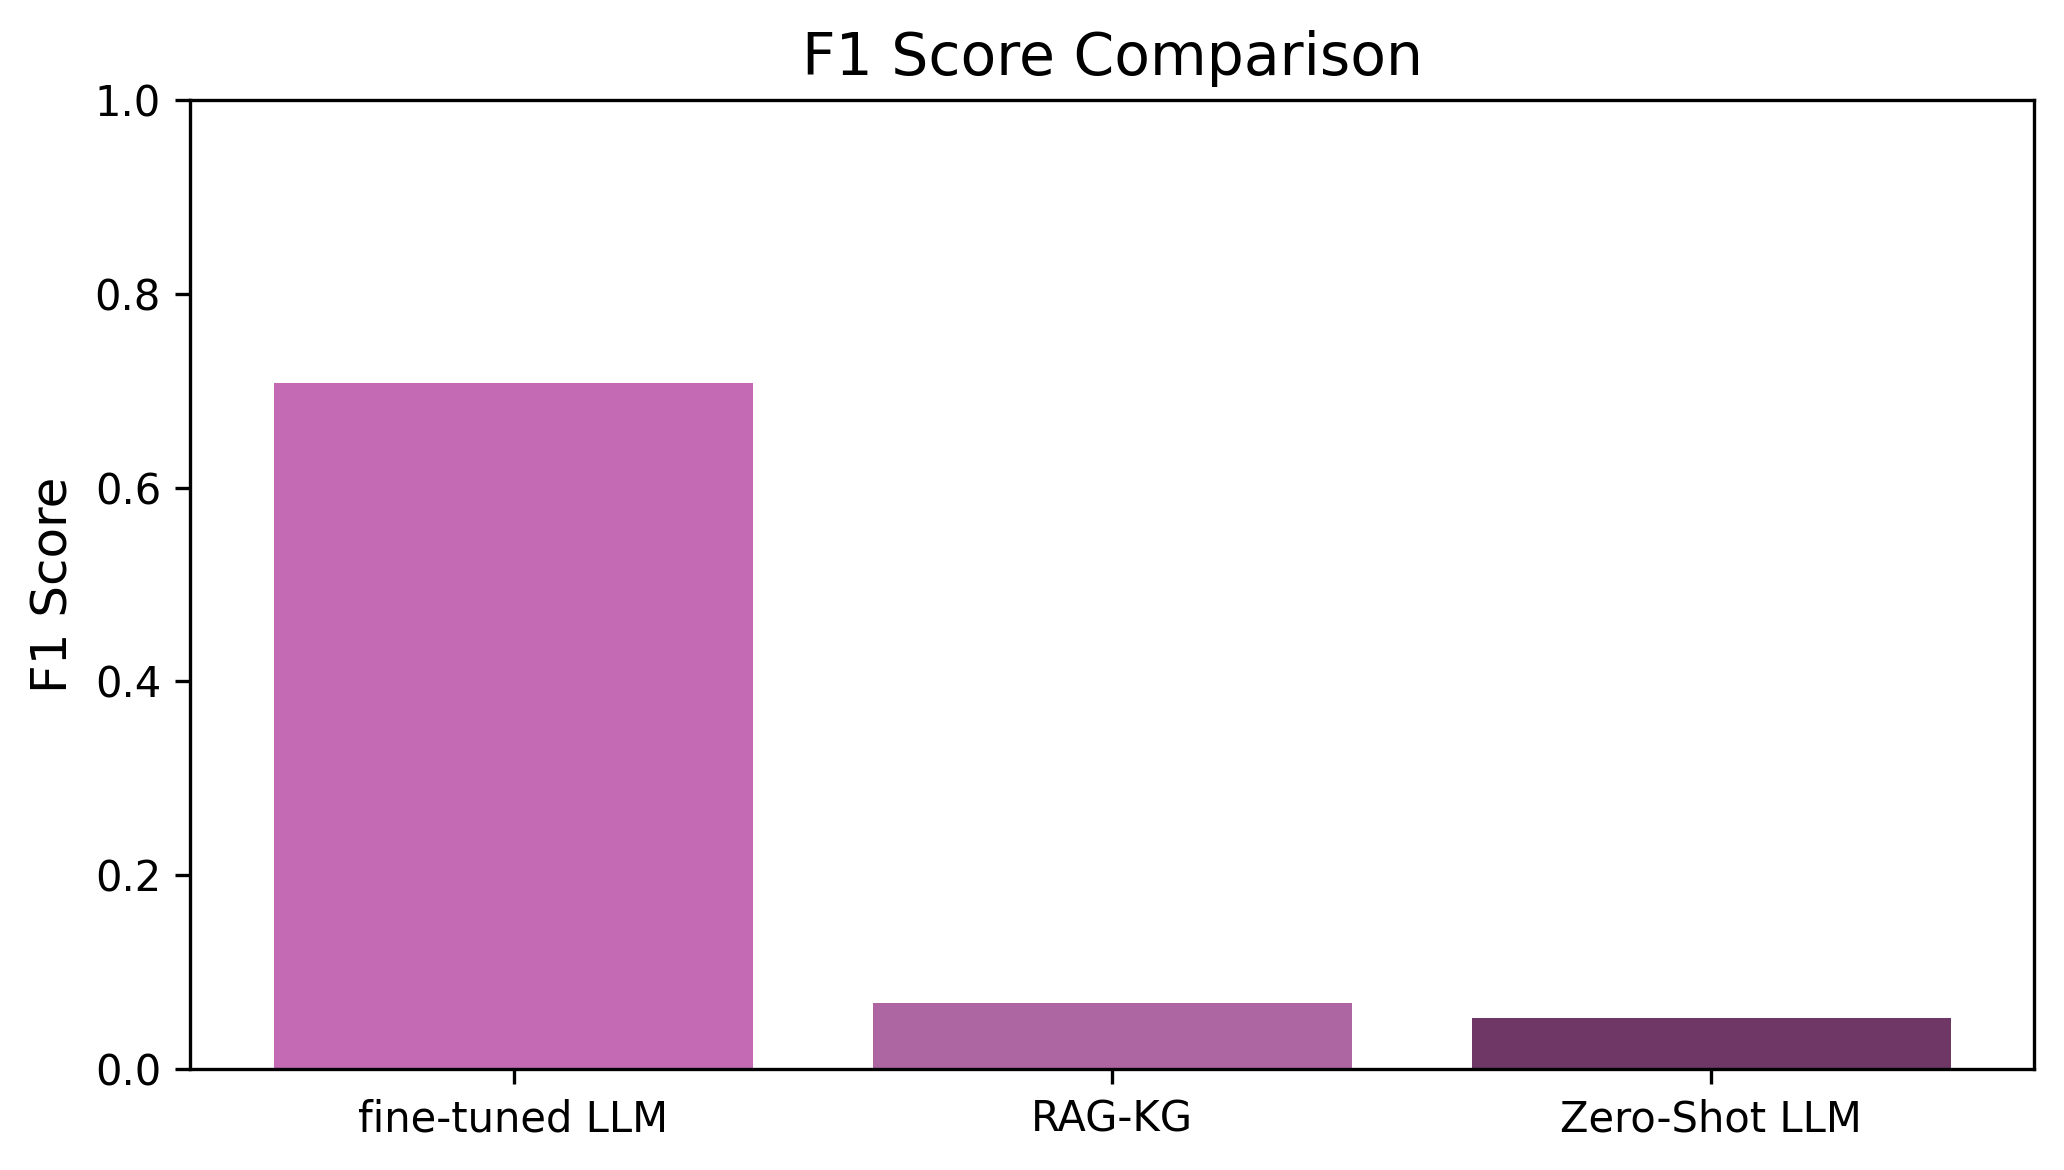
\includegraphics[width=\columnwidth]{images/eval/evaluation_comparison_f1_score_2.png}
    \caption{F1 scores on three comparison models.}
    \label{fig:f1_score}
\end{figure}

\begin{figure}[h!]
    \centering
    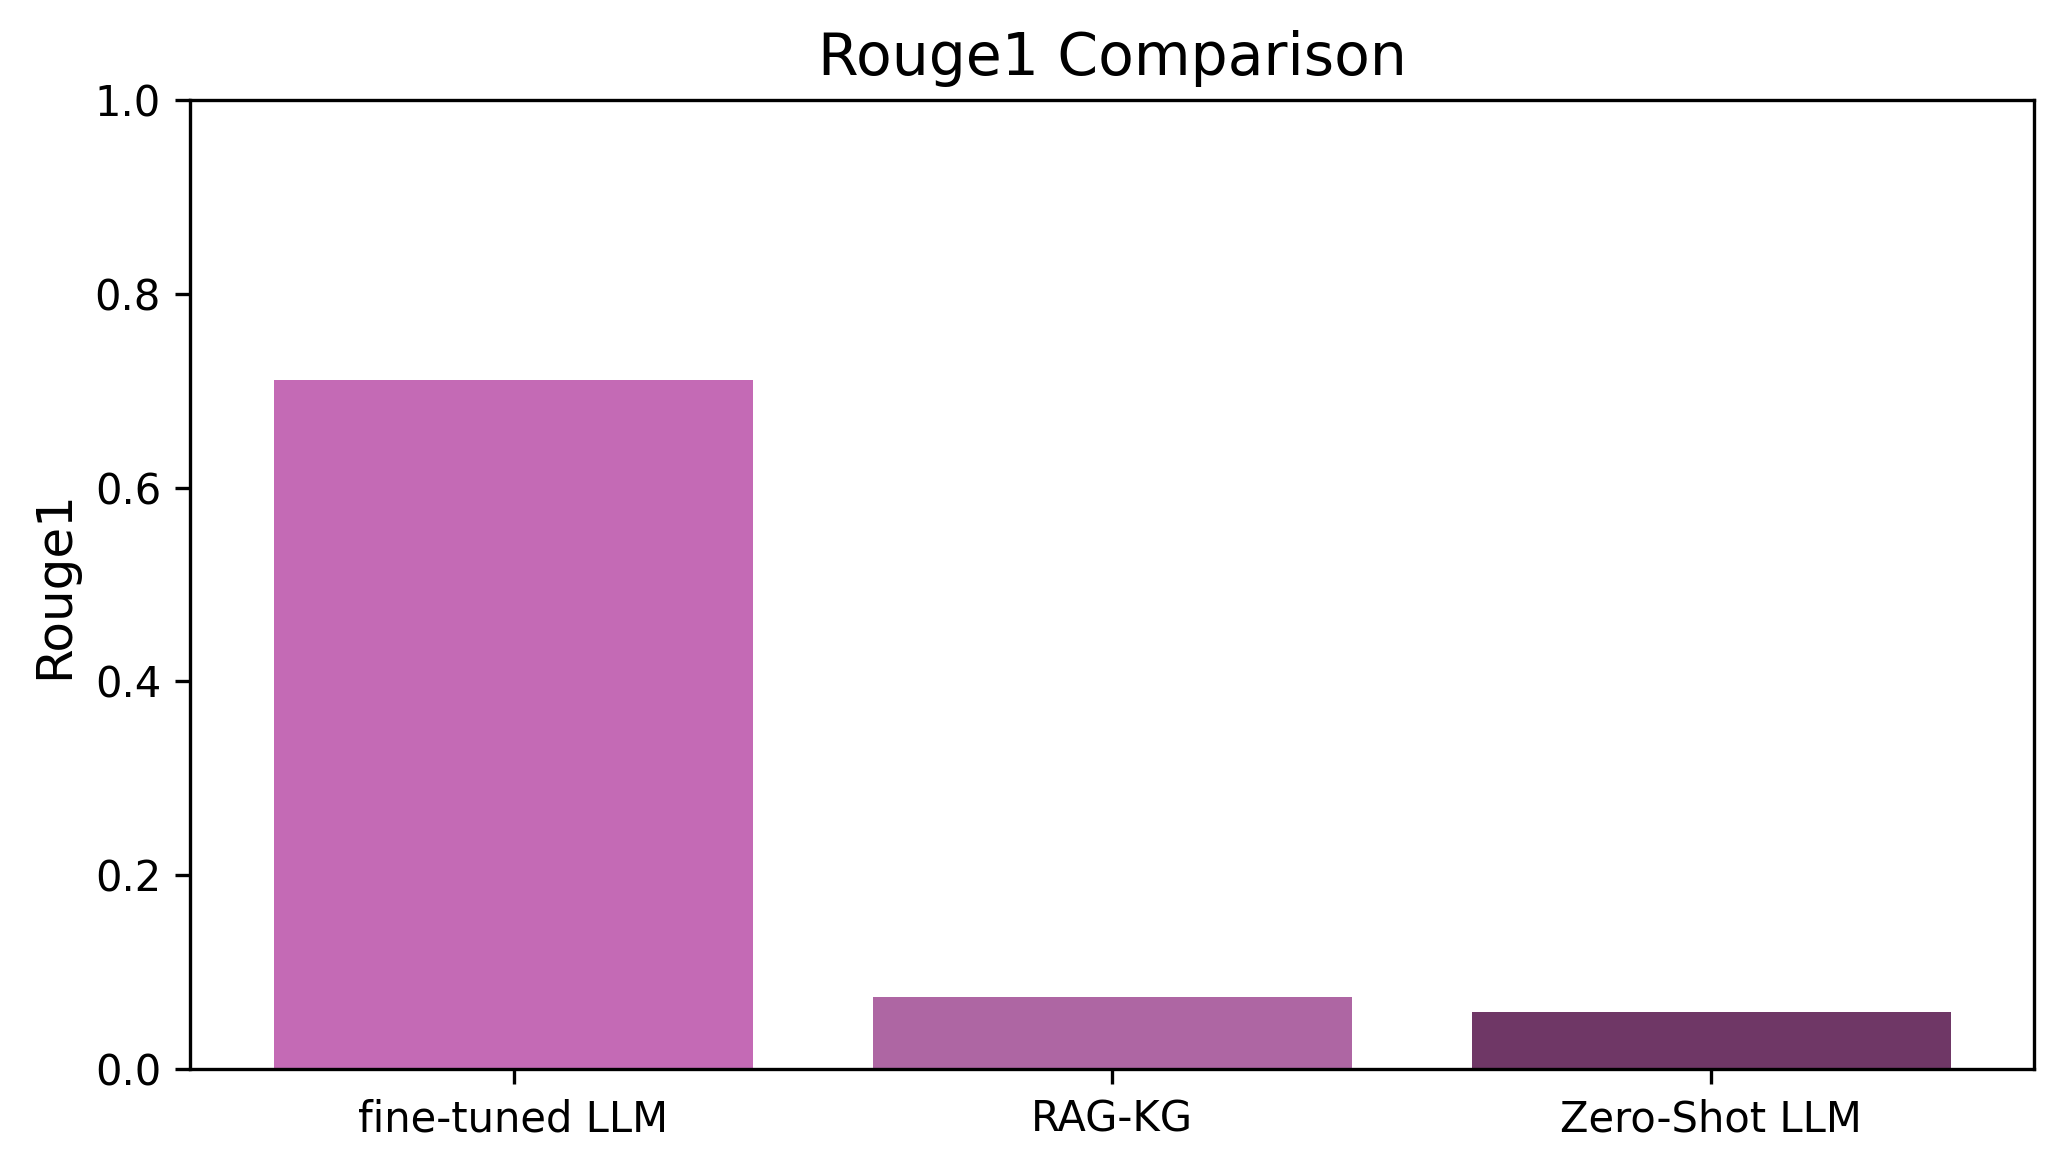
\includegraphics[width=\columnwidth]{images/eval/evaluation_comparison_rouge1_2.png}
    \caption{ROUGE1 scores on three comparison models.}
    \label{fig:rouge1}
\end{figure}

\begin{figure}[h!]
    \centering
    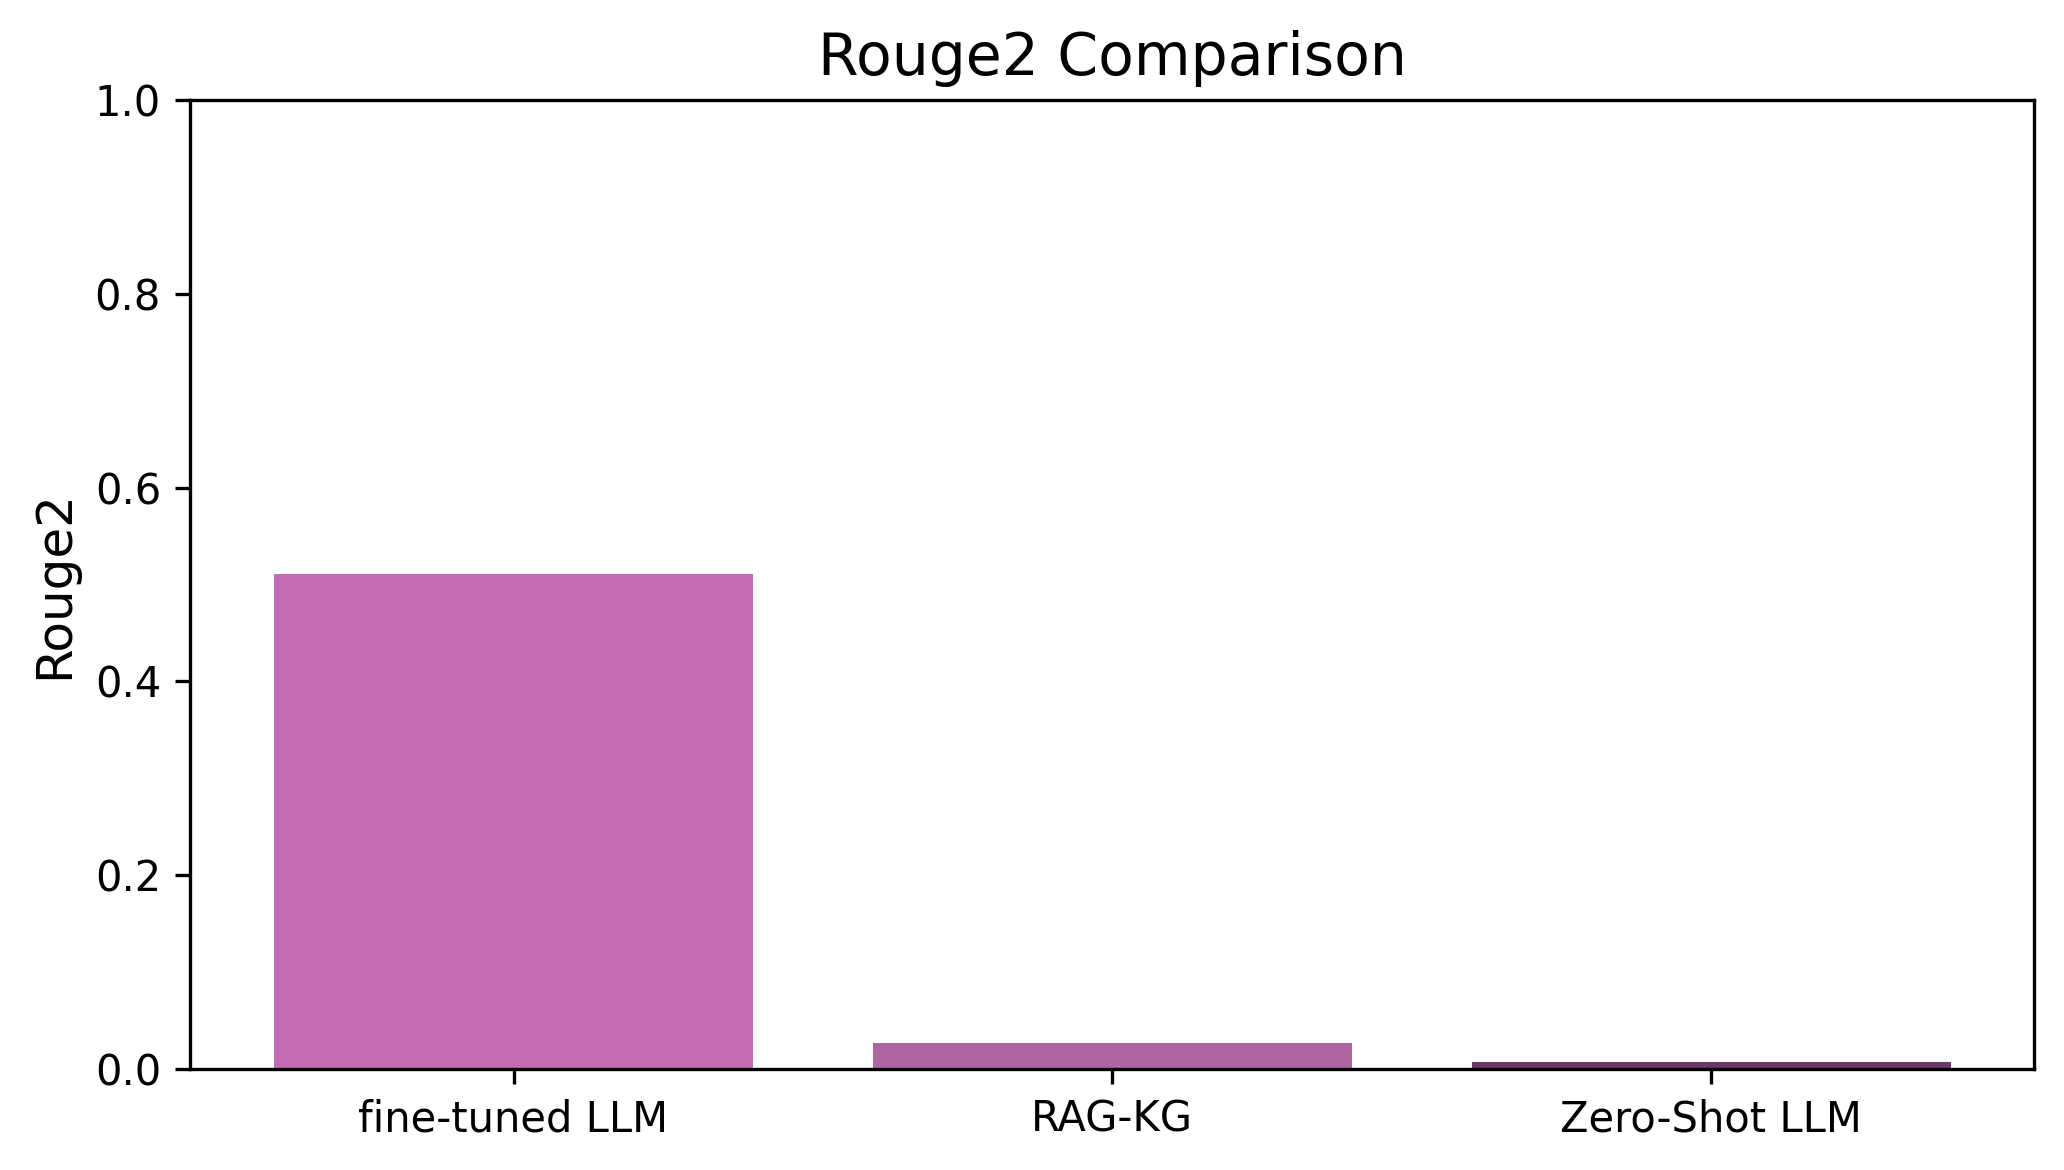
\includegraphics[width=\columnwidth]{images/eval/evaluation_comparison_rouge2_2.png}
    \caption{ROUGE2 scores on three comparison models.}
    \label{fig:rouge2}
\end{figure}

\begin{figure}[h!]
    \centering
    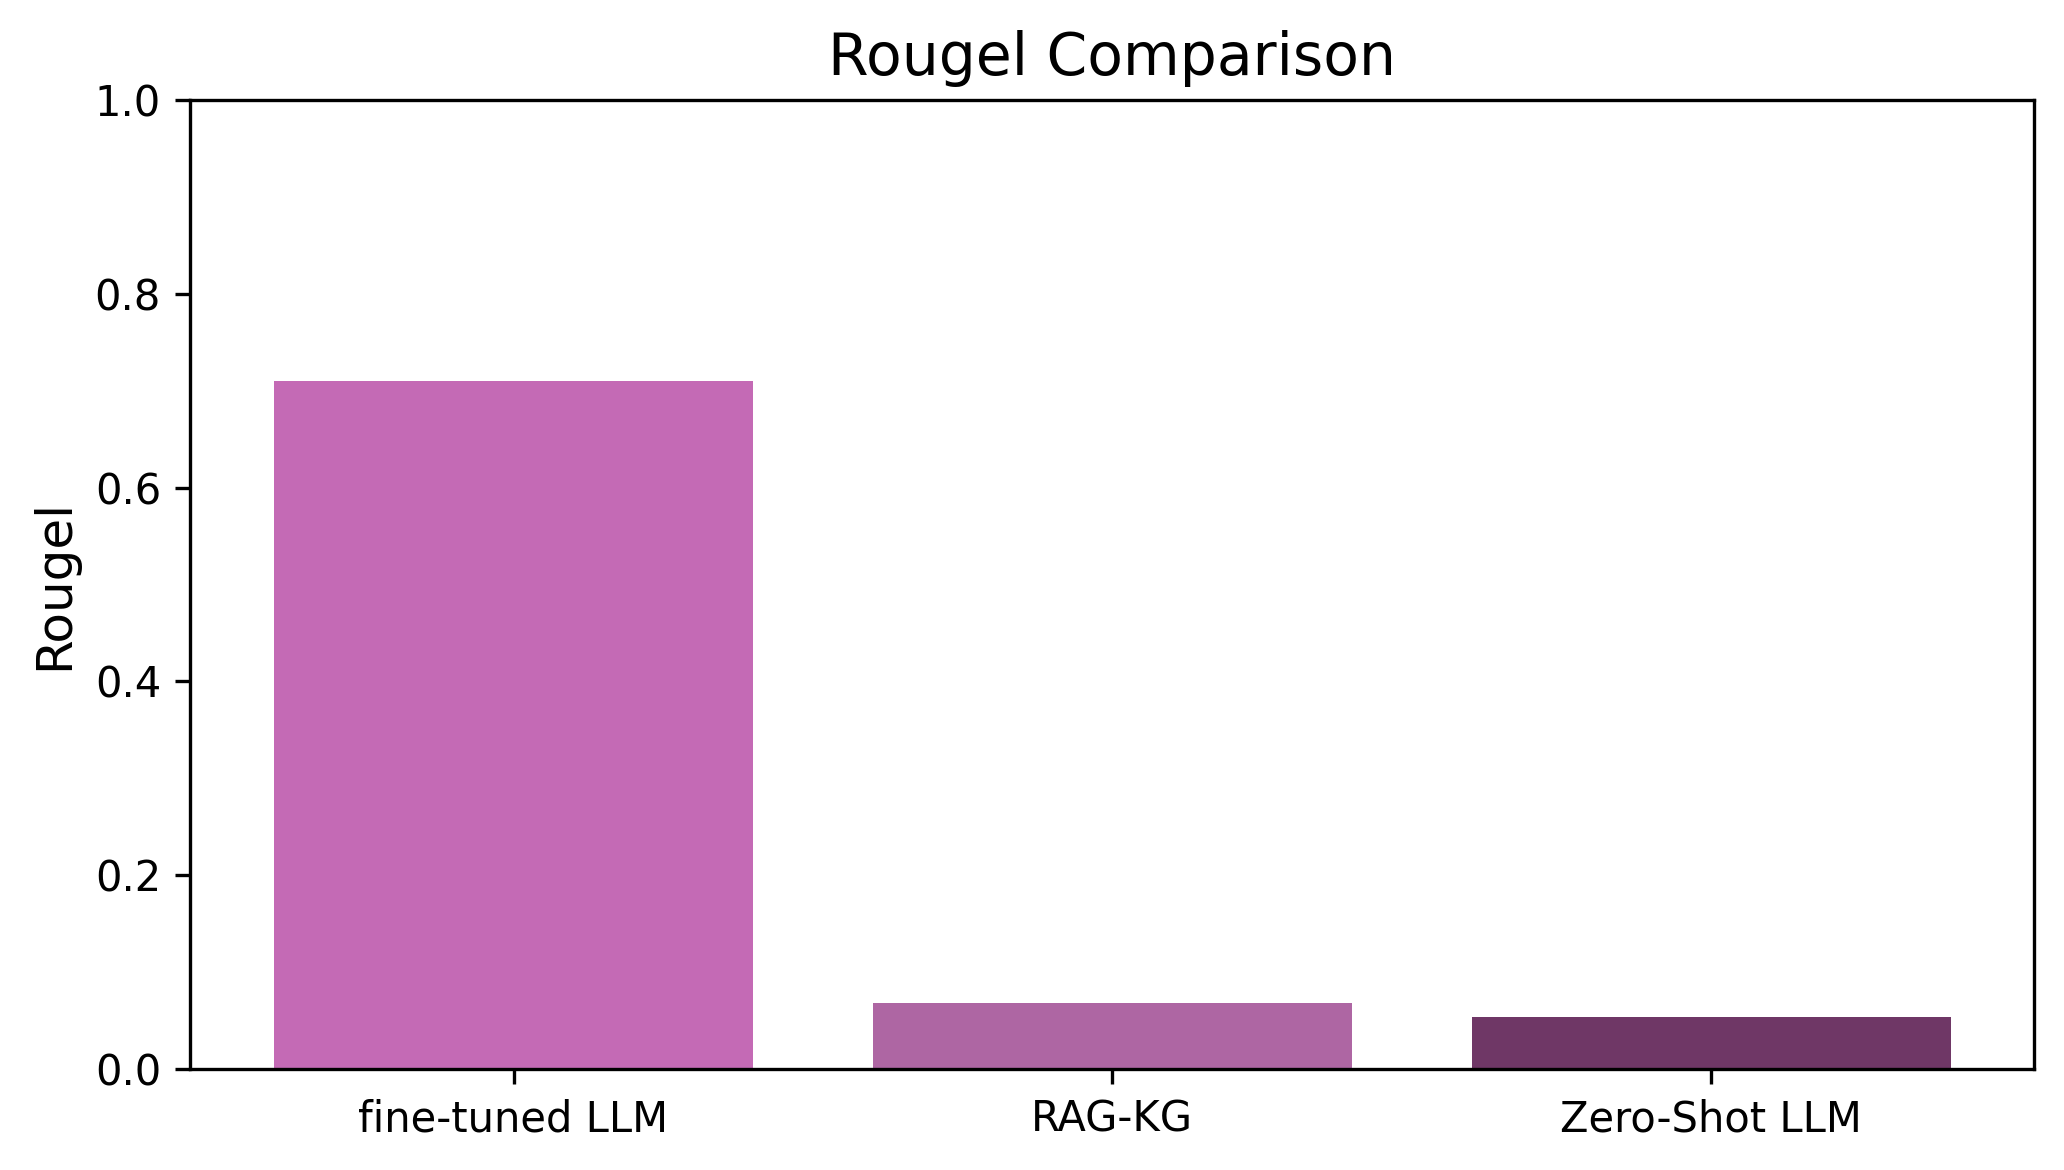
\includegraphics[width=\columnwidth]{images/eval/evaluation_comparison_rougeL_2.png}
    \caption{ROUGEL scores on three comparison models.}
    \label{fig:rougeL}
\end{figure}

\begin{figure}[h!]
    \centering
    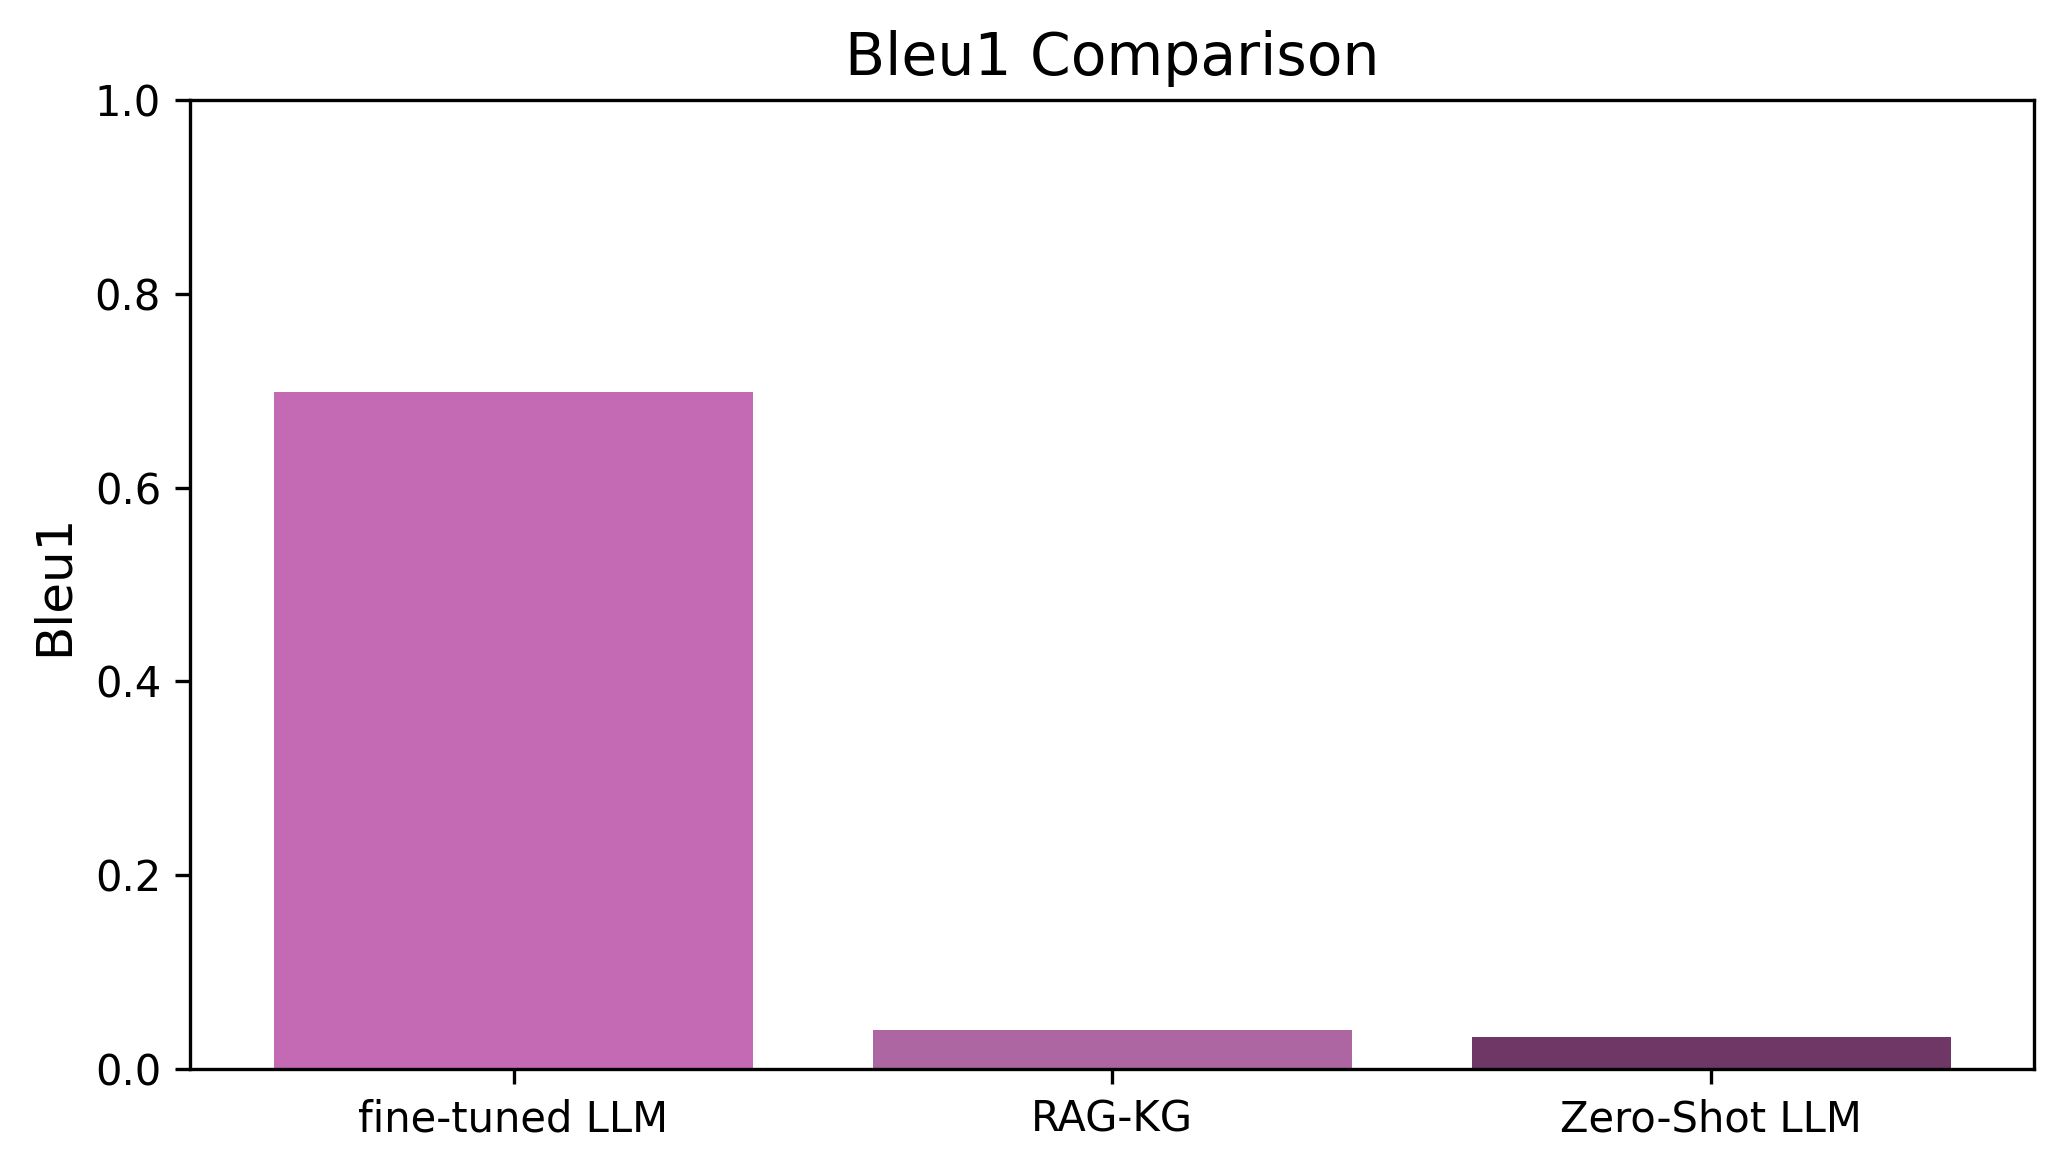
\includegraphics[width=\columnwidth]{images/eval/evaluation_comparison_bleu1_2.png}
    \caption{BLEU1 scores on three comparison models.}
    \label{fig:bleu1}
\end{figure}

\begin{figure}[h!]
    \centering
    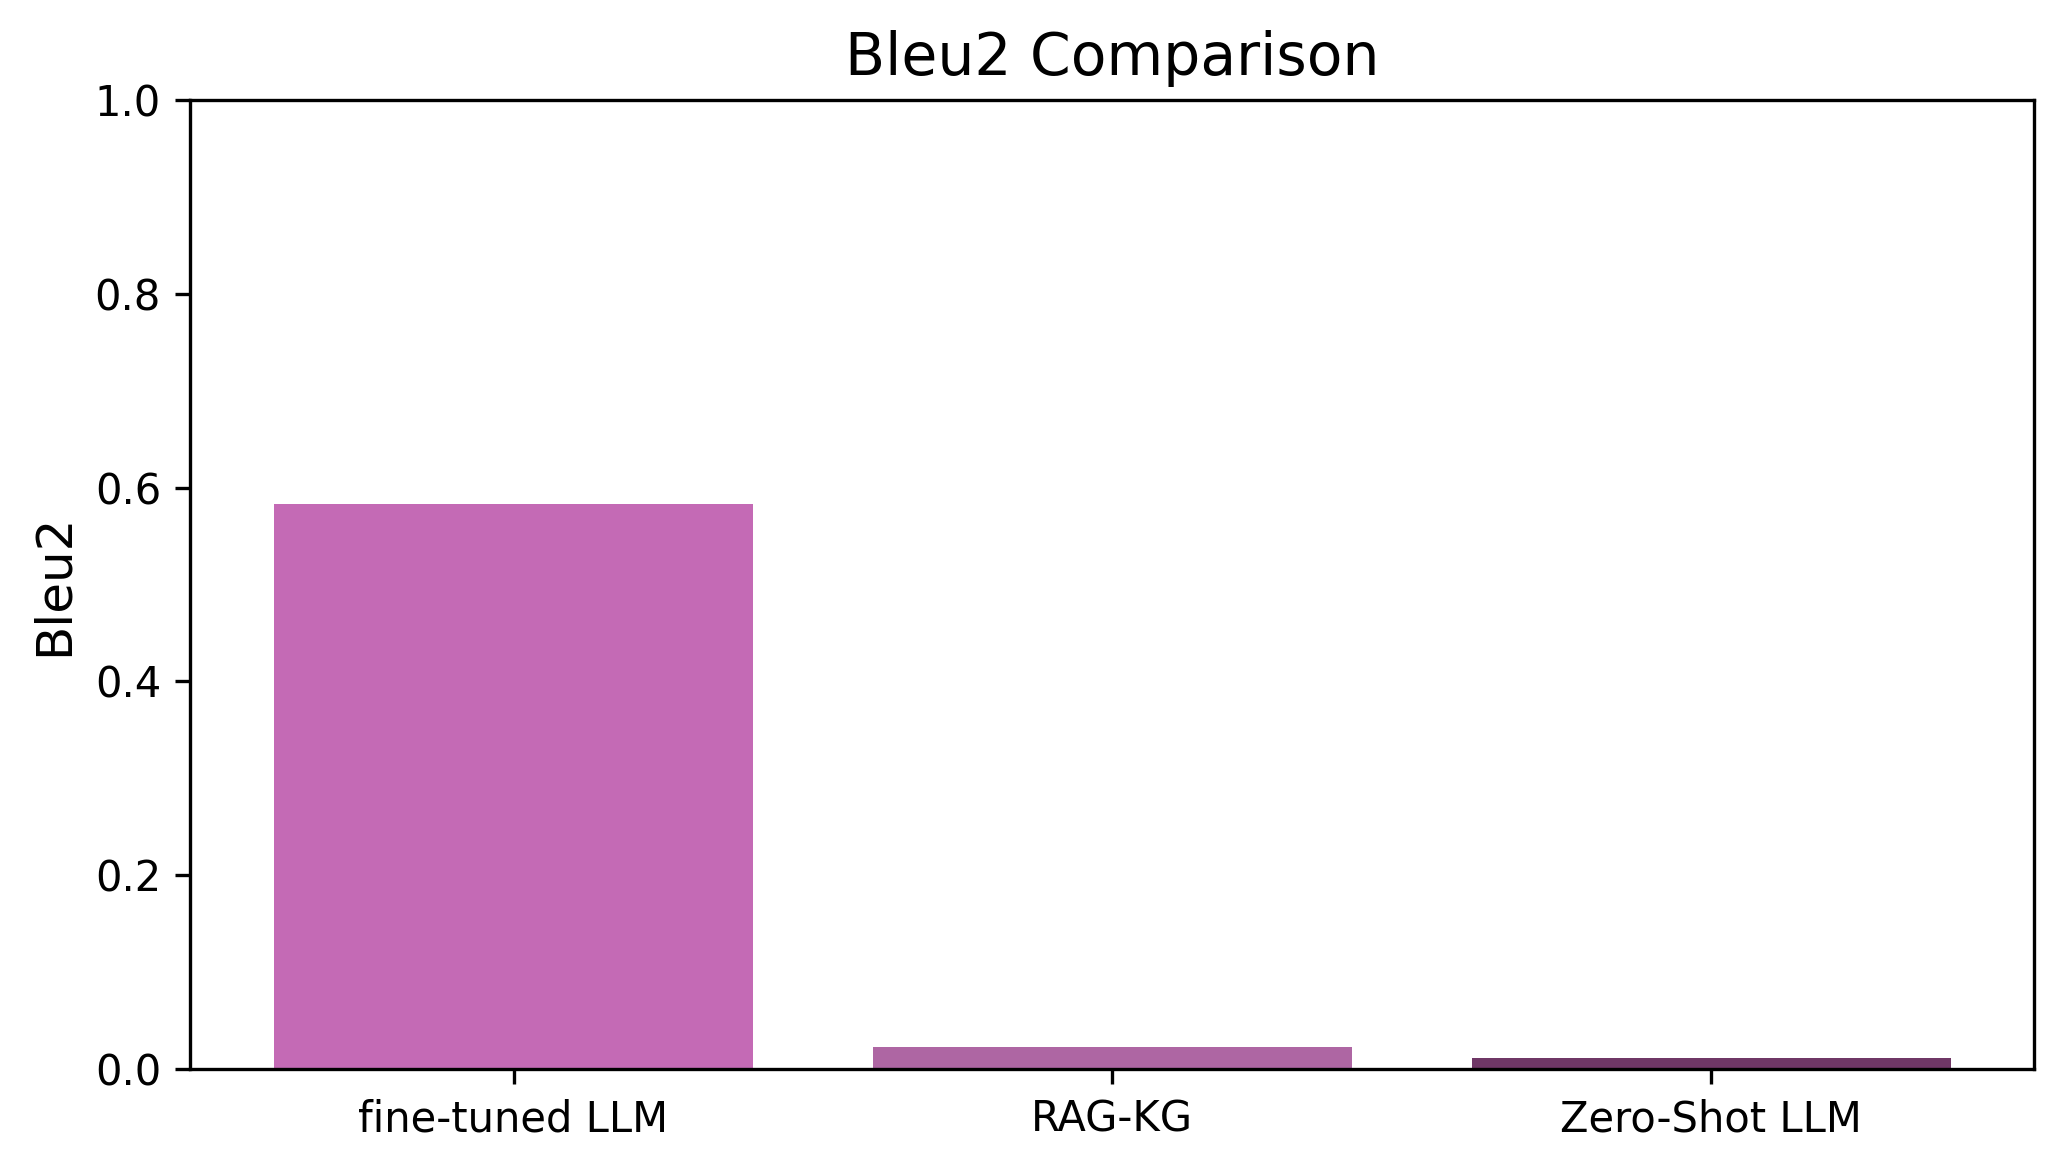
\includegraphics[width=\columnwidth]{images/eval/evaluation_comparison_bleu2_2.png}
    \caption{BLEU2 scores on three comparison models.}
    \label{fig:bleu2}
\end{figure}

\begin{figure}[h!]
    \centering
    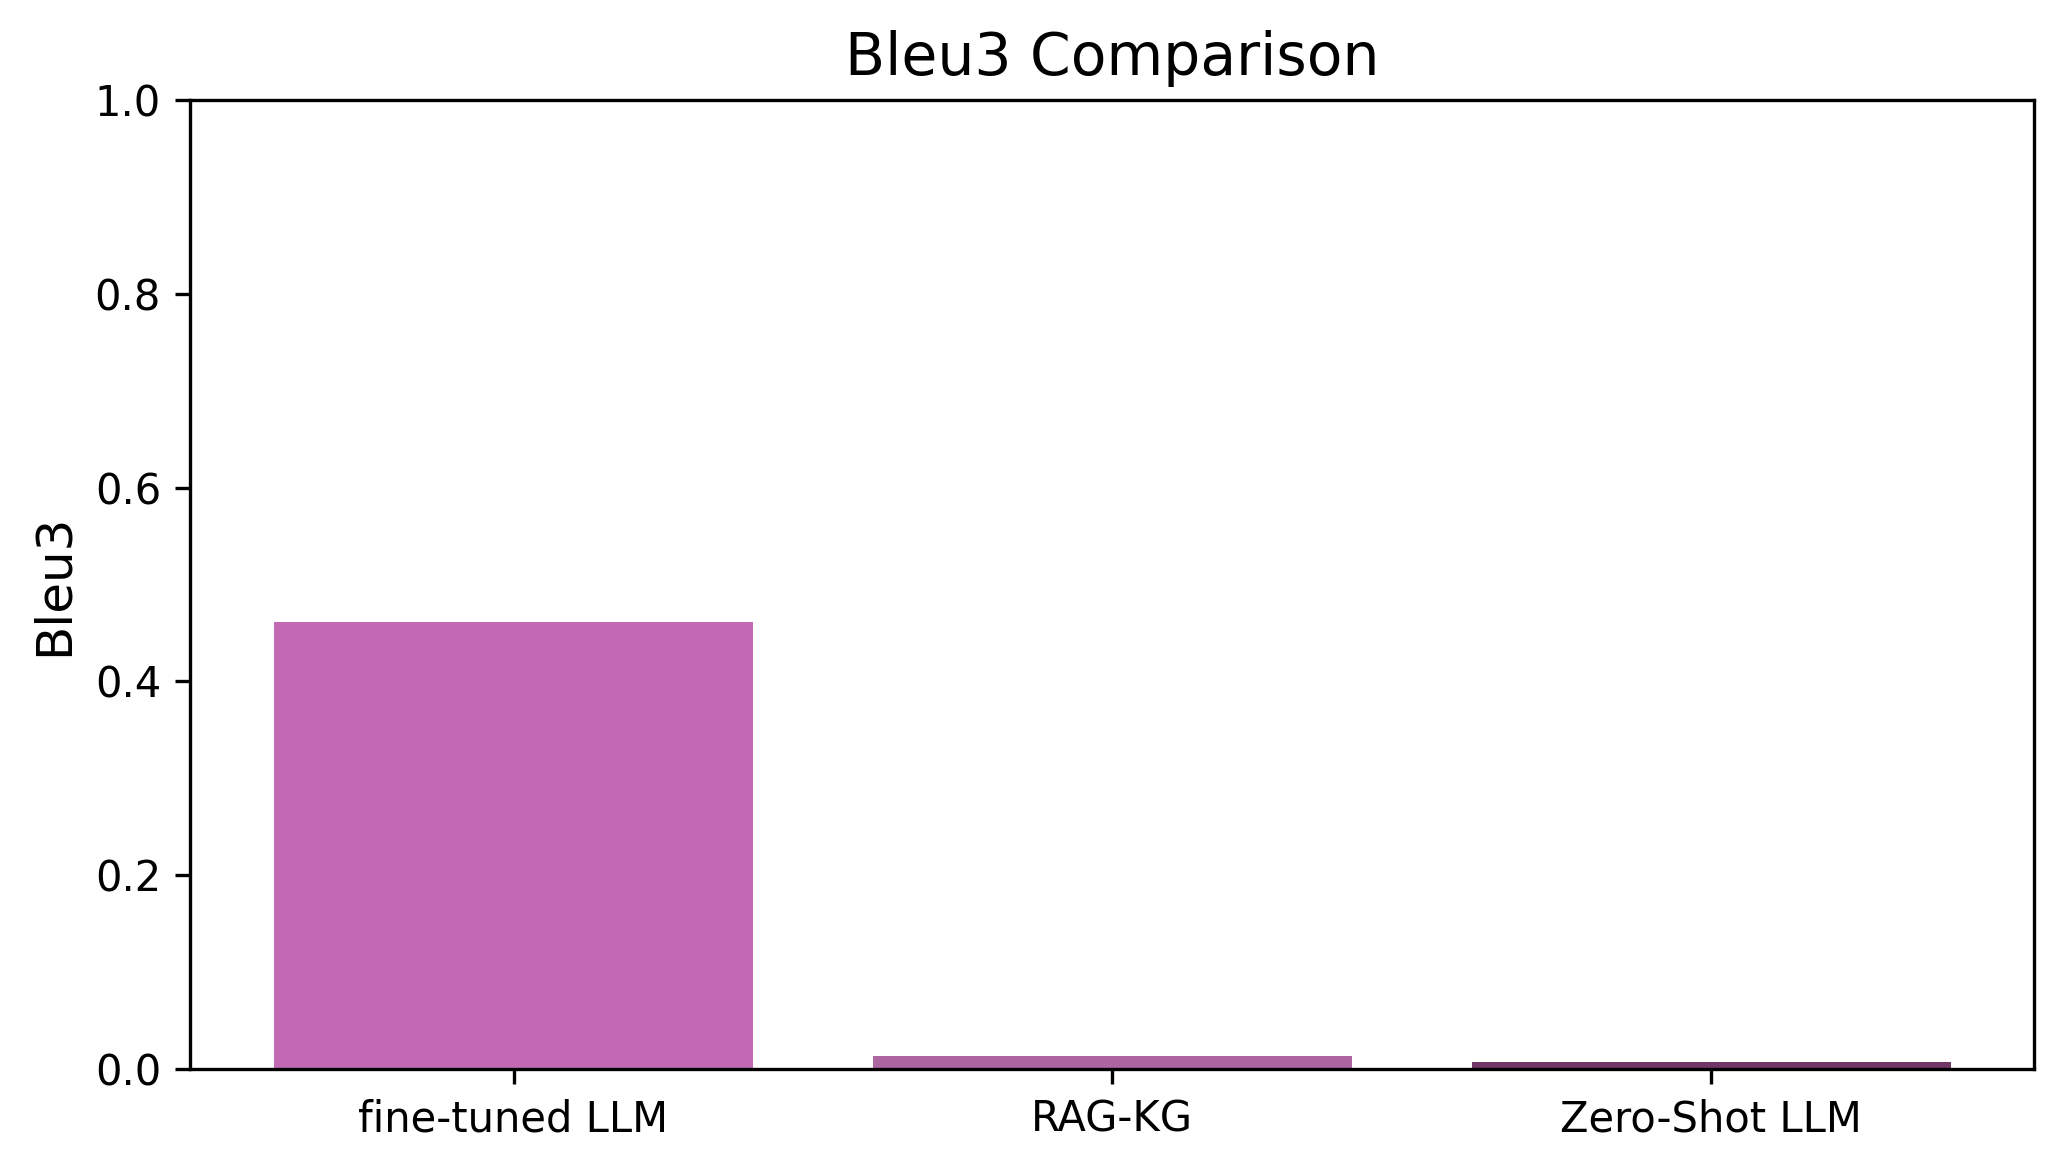
\includegraphics[width=\columnwidth]{images/eval/evaluation_comparison_bleu3_2.png}
    \caption{BLEU3 scores on three comparison models.}
    \label{fig:bleu3}
\end{figure}

\begin{figure}[h!]
    \centering
    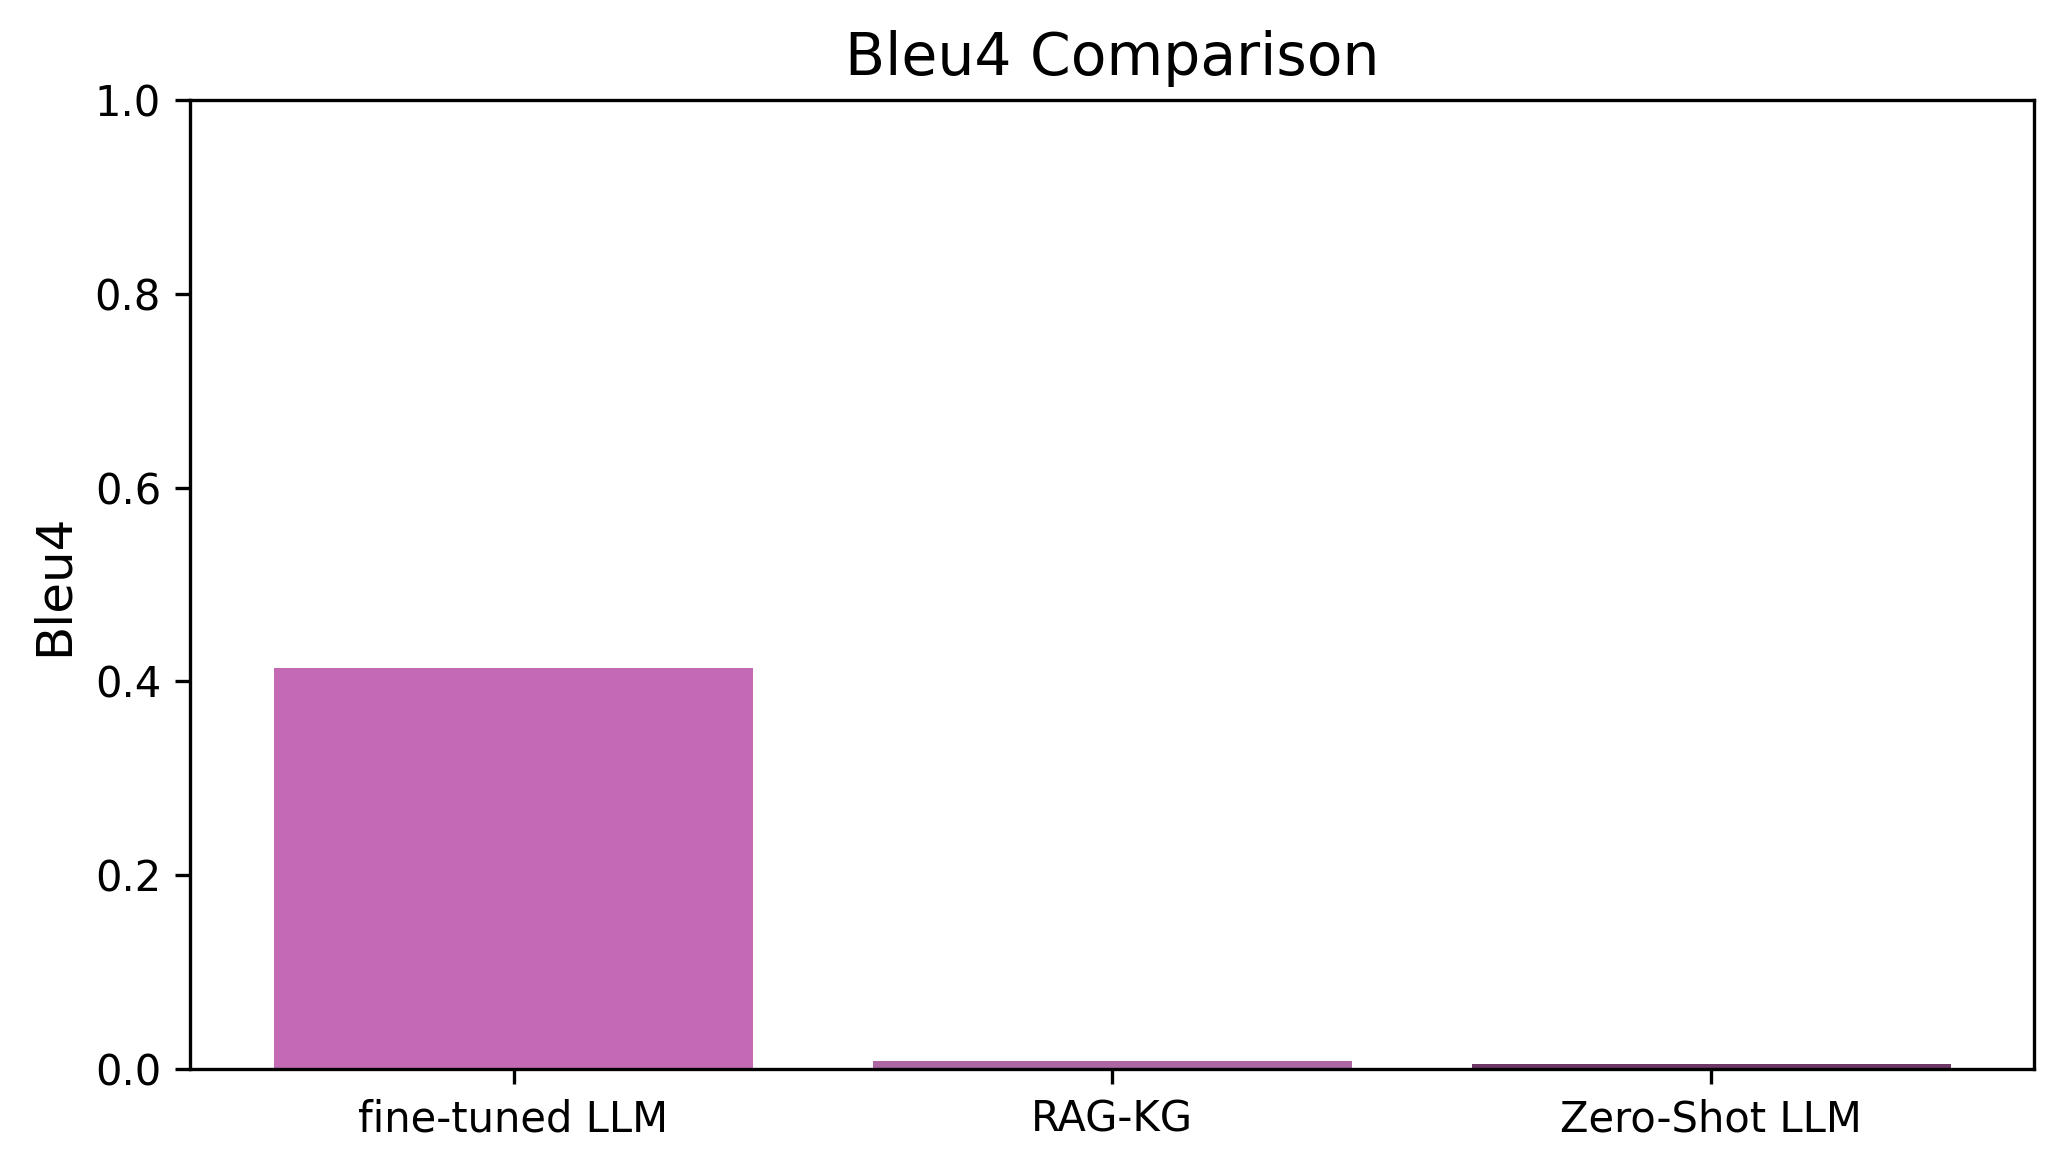
\includegraphics[width=\columnwidth]{images/eval/evaluation_comparison_bleu4_2.png}
    \caption{BLEU4 scores on three comparison models.}
    \label{fig:bleu4}
\end{figure}

Figure~\ref{fig:const_sat} shows the constraint satisfaction rate of the three models. A deeper manual evaluation reveals that the lower performance of the fine-tuned LLM stems from its tendency to include as much relevant information as possible, such as listing three food nutrients when only two are required.

\begin{figure}[h!]
    \centering
    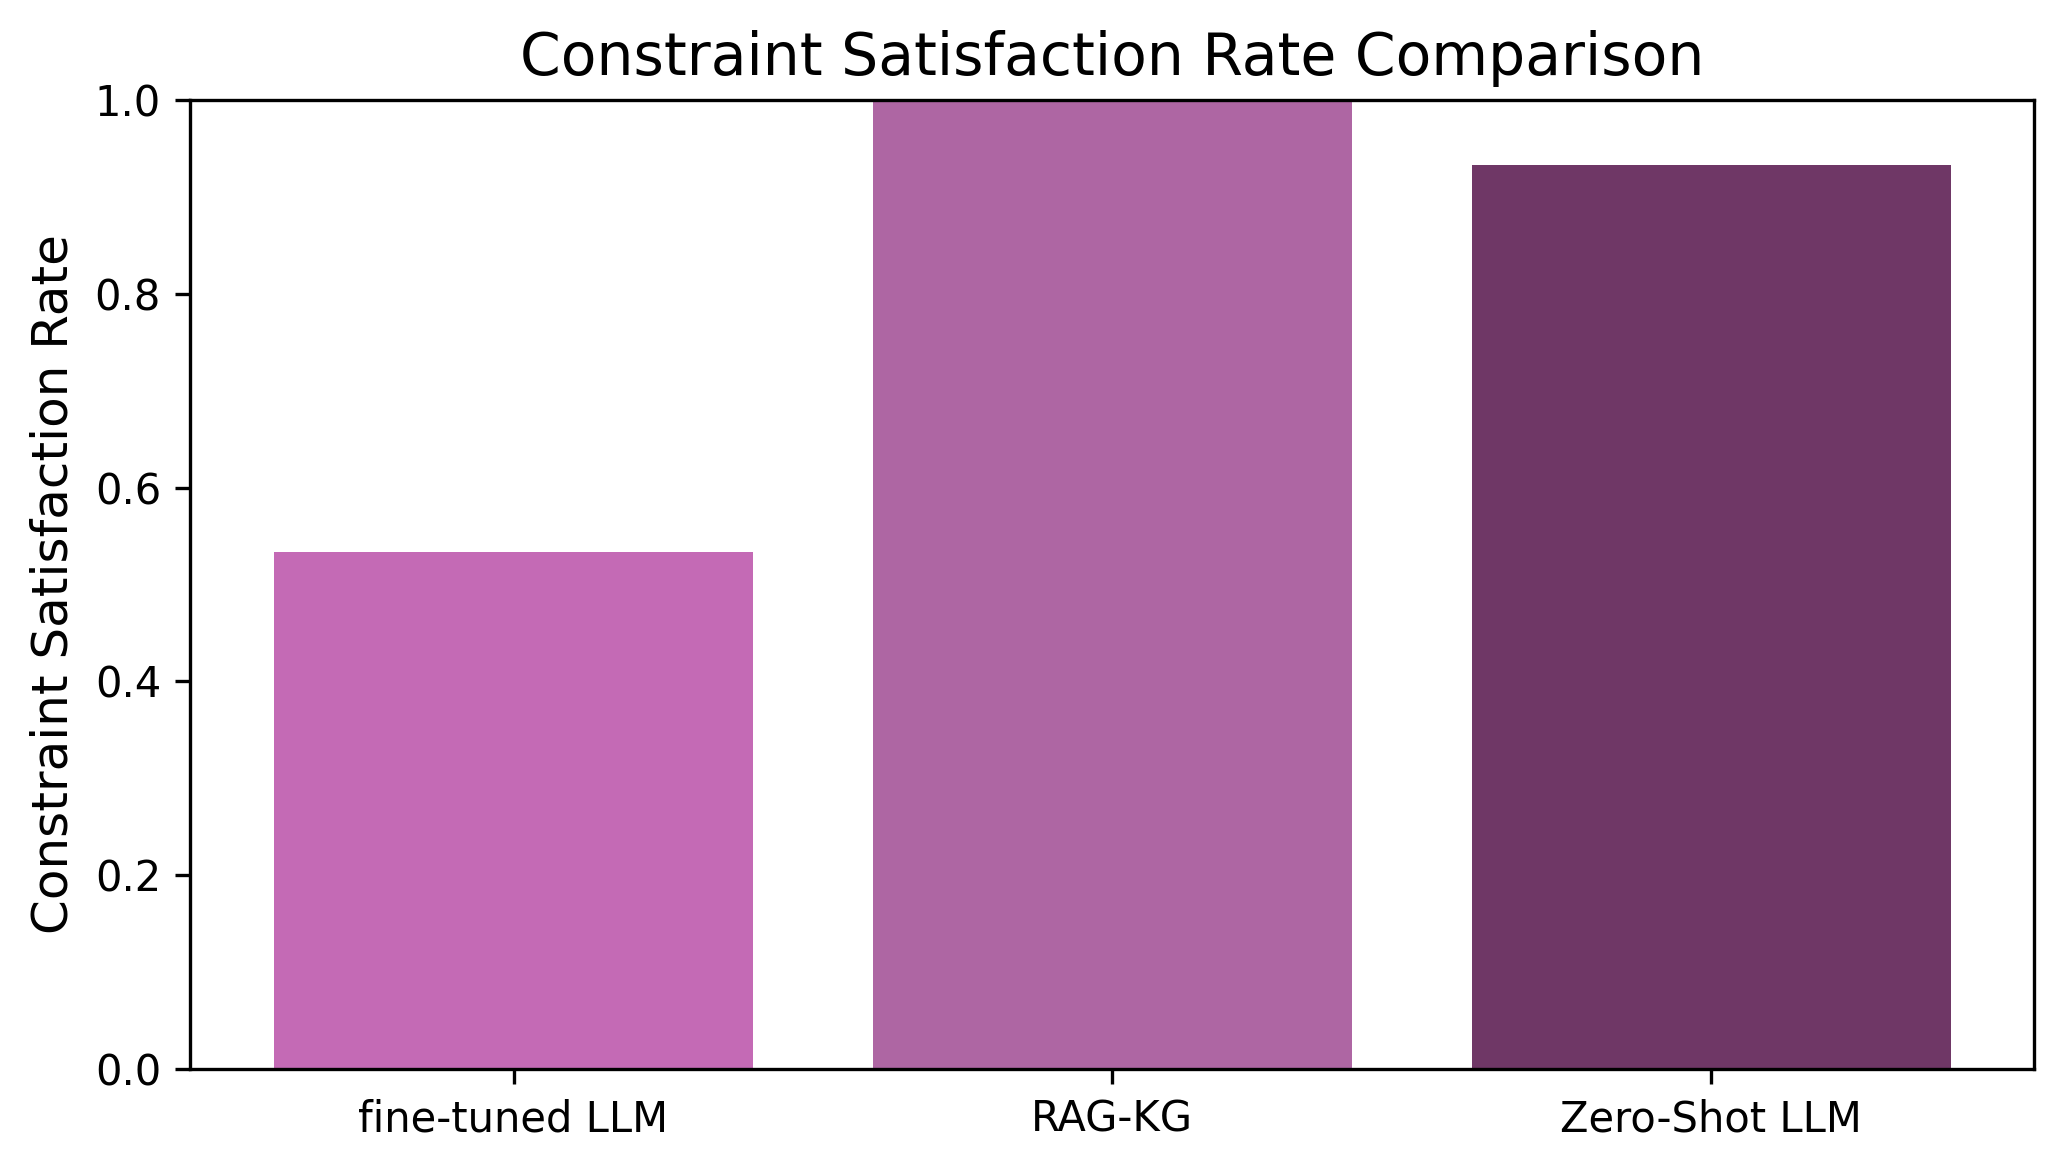
\includegraphics[width=\columnwidth]{images/eval/evaluation_comparison_constraint_satisfaction_rate_2.png}
    \caption{Constraint satisfaction rate on three comparison models.}
    \label{fig:const_sat}
\end{figure}

These results are strongly skewed in favor of the fine-tuned model partly because it is the only one trained on data written in the same format as the answers in the test set, and is therefore able to reproduce the expected output structure with higher coherence. In contrast, automatic metrics are not capable of reliably assessing the semantic correctness or completeness of an answer: a response may be accurate from a content perspective, but if written in a different format (e.g., more verbose or narrative), it may receive very low scores under metrics such as F1 score.

Moreover, several instructions in the test set admitted more than one valid answer. In such cases, any response that was correct but different from the reference answer negatively affected the automatic metric results, further penalizing models that generated plausible yet non-identical outputs.

After a combined manual evaluation and an external LLM-based assessment, it was confirmed that the fine-tuned model achieves performance comparable to, or better than, both the RAG-KG model and the zero-shot LLM, despite having been trained on only a single data source (a PDF document). As shown in Figures~\ref{fig:relevance},~\ref{fig:completeness} and ~\ref{fig:citation} the rubric-based metrics confirmed the reliability and overall quality of the fine-tuned model’s outputs.

\begin{figure}[h!]
    \centering
    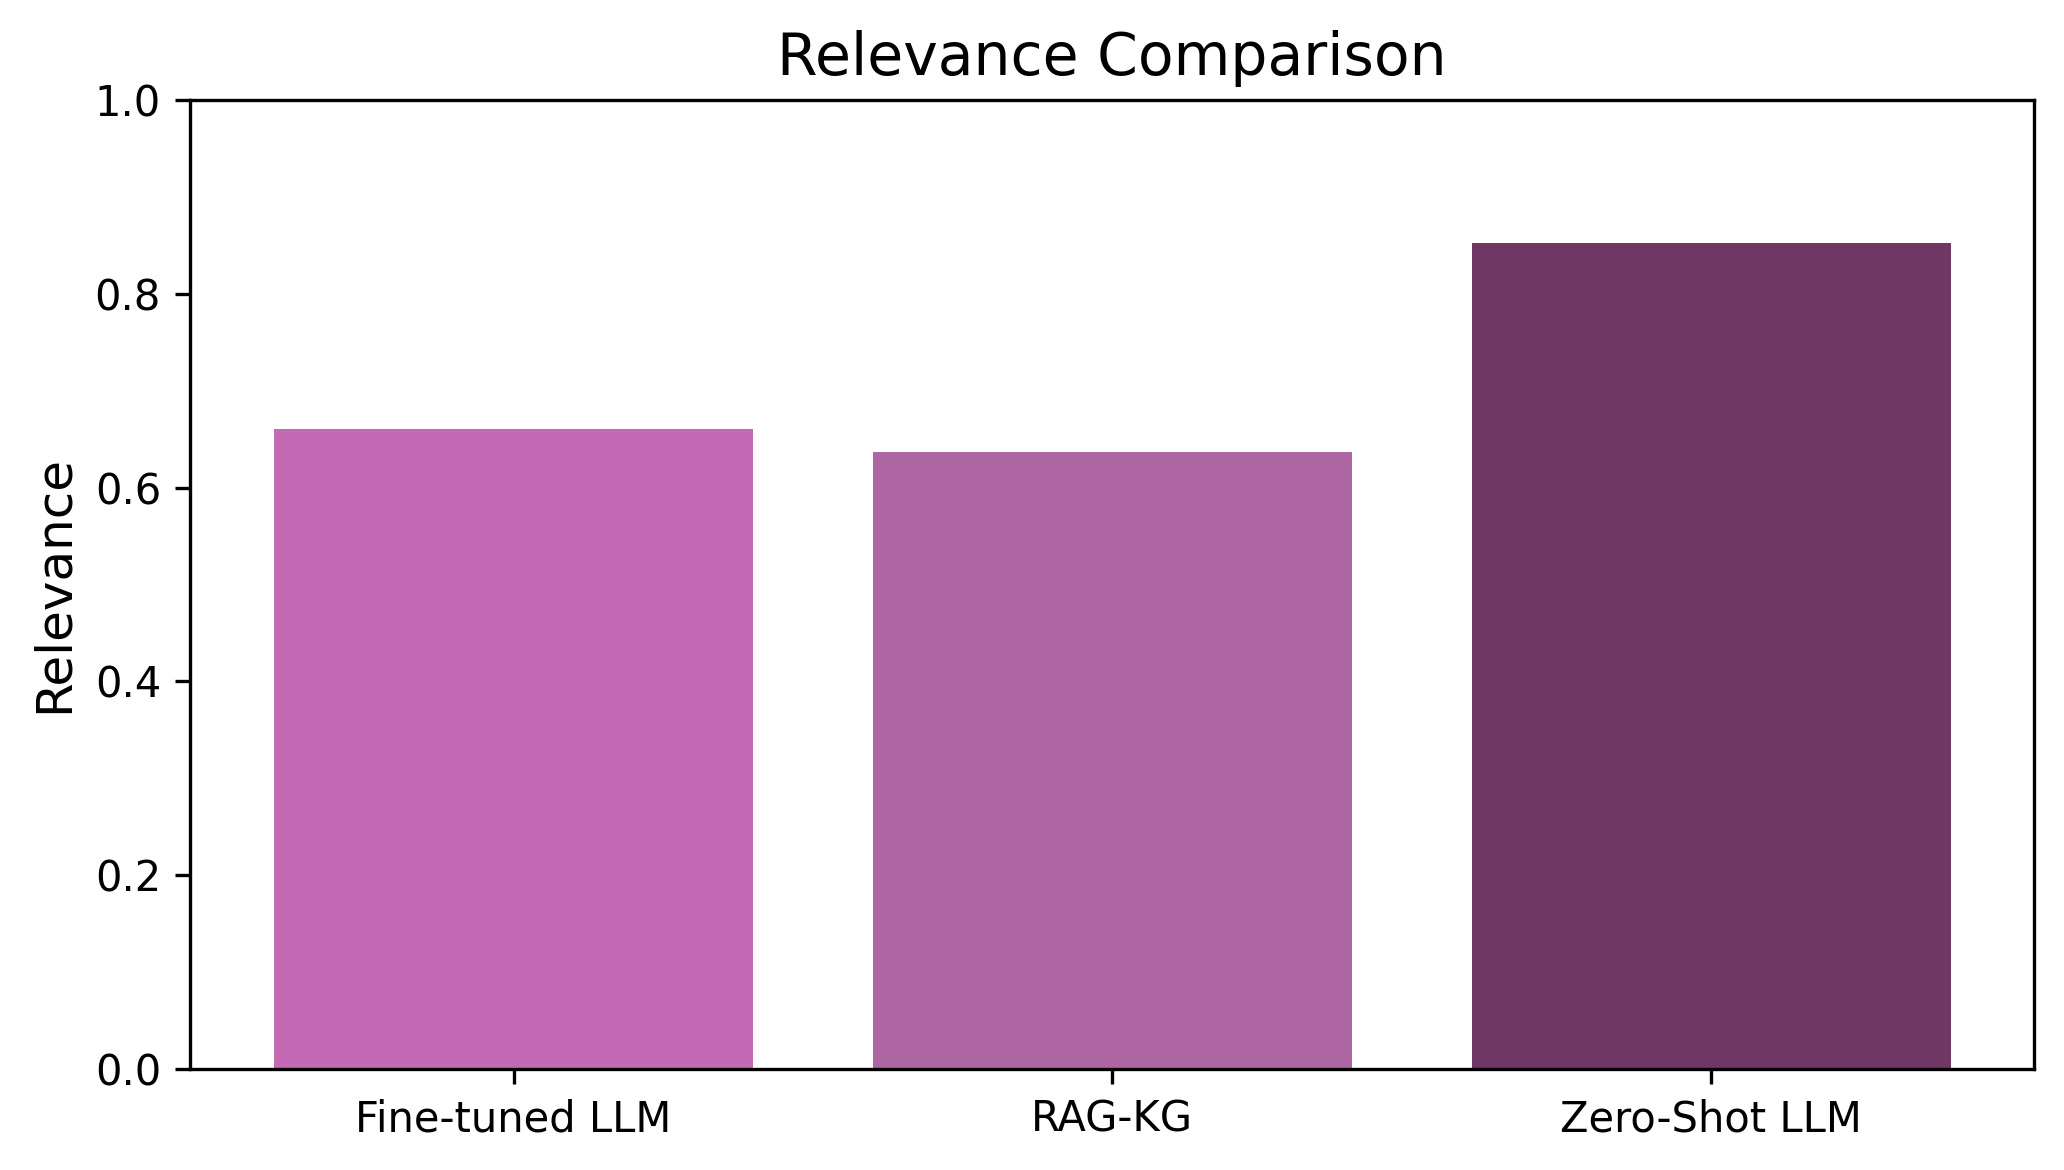
\includegraphics[width=\columnwidth]{images/eval/groq_comparison_relevance_2.png}
    \caption{Relevance on three comparison models.}
    \label{fig:relevance}
\end{figure}

\begin{figure}[h!]
    \centering
    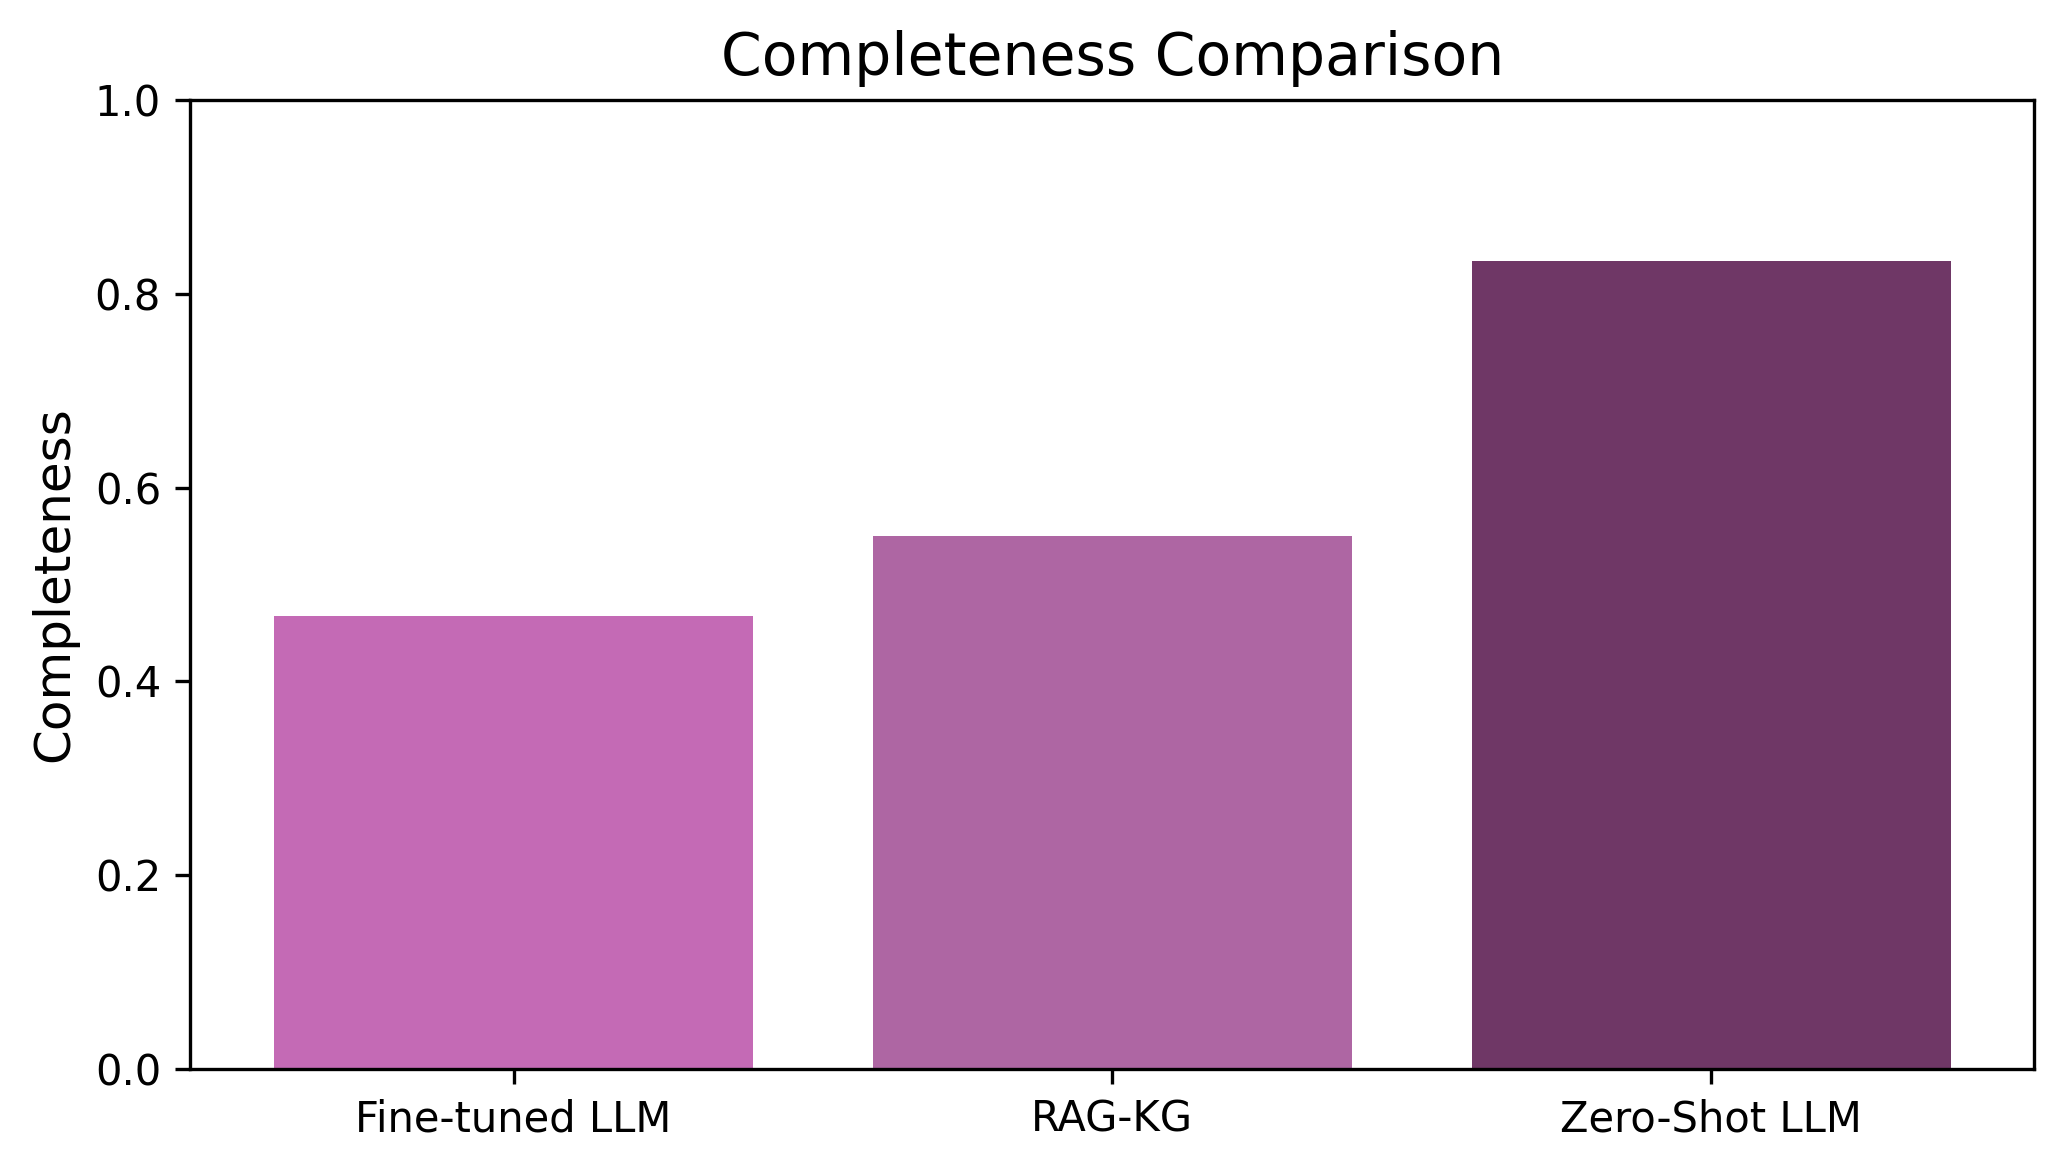
\includegraphics[width=\columnwidth]{images/eval/groq_comparison_completeness_2.png}
    \caption{Completeness on three comparison models.}
    \label{fig:completeness}
\end{figure}

\begin{figure}[h!]
    \centering
    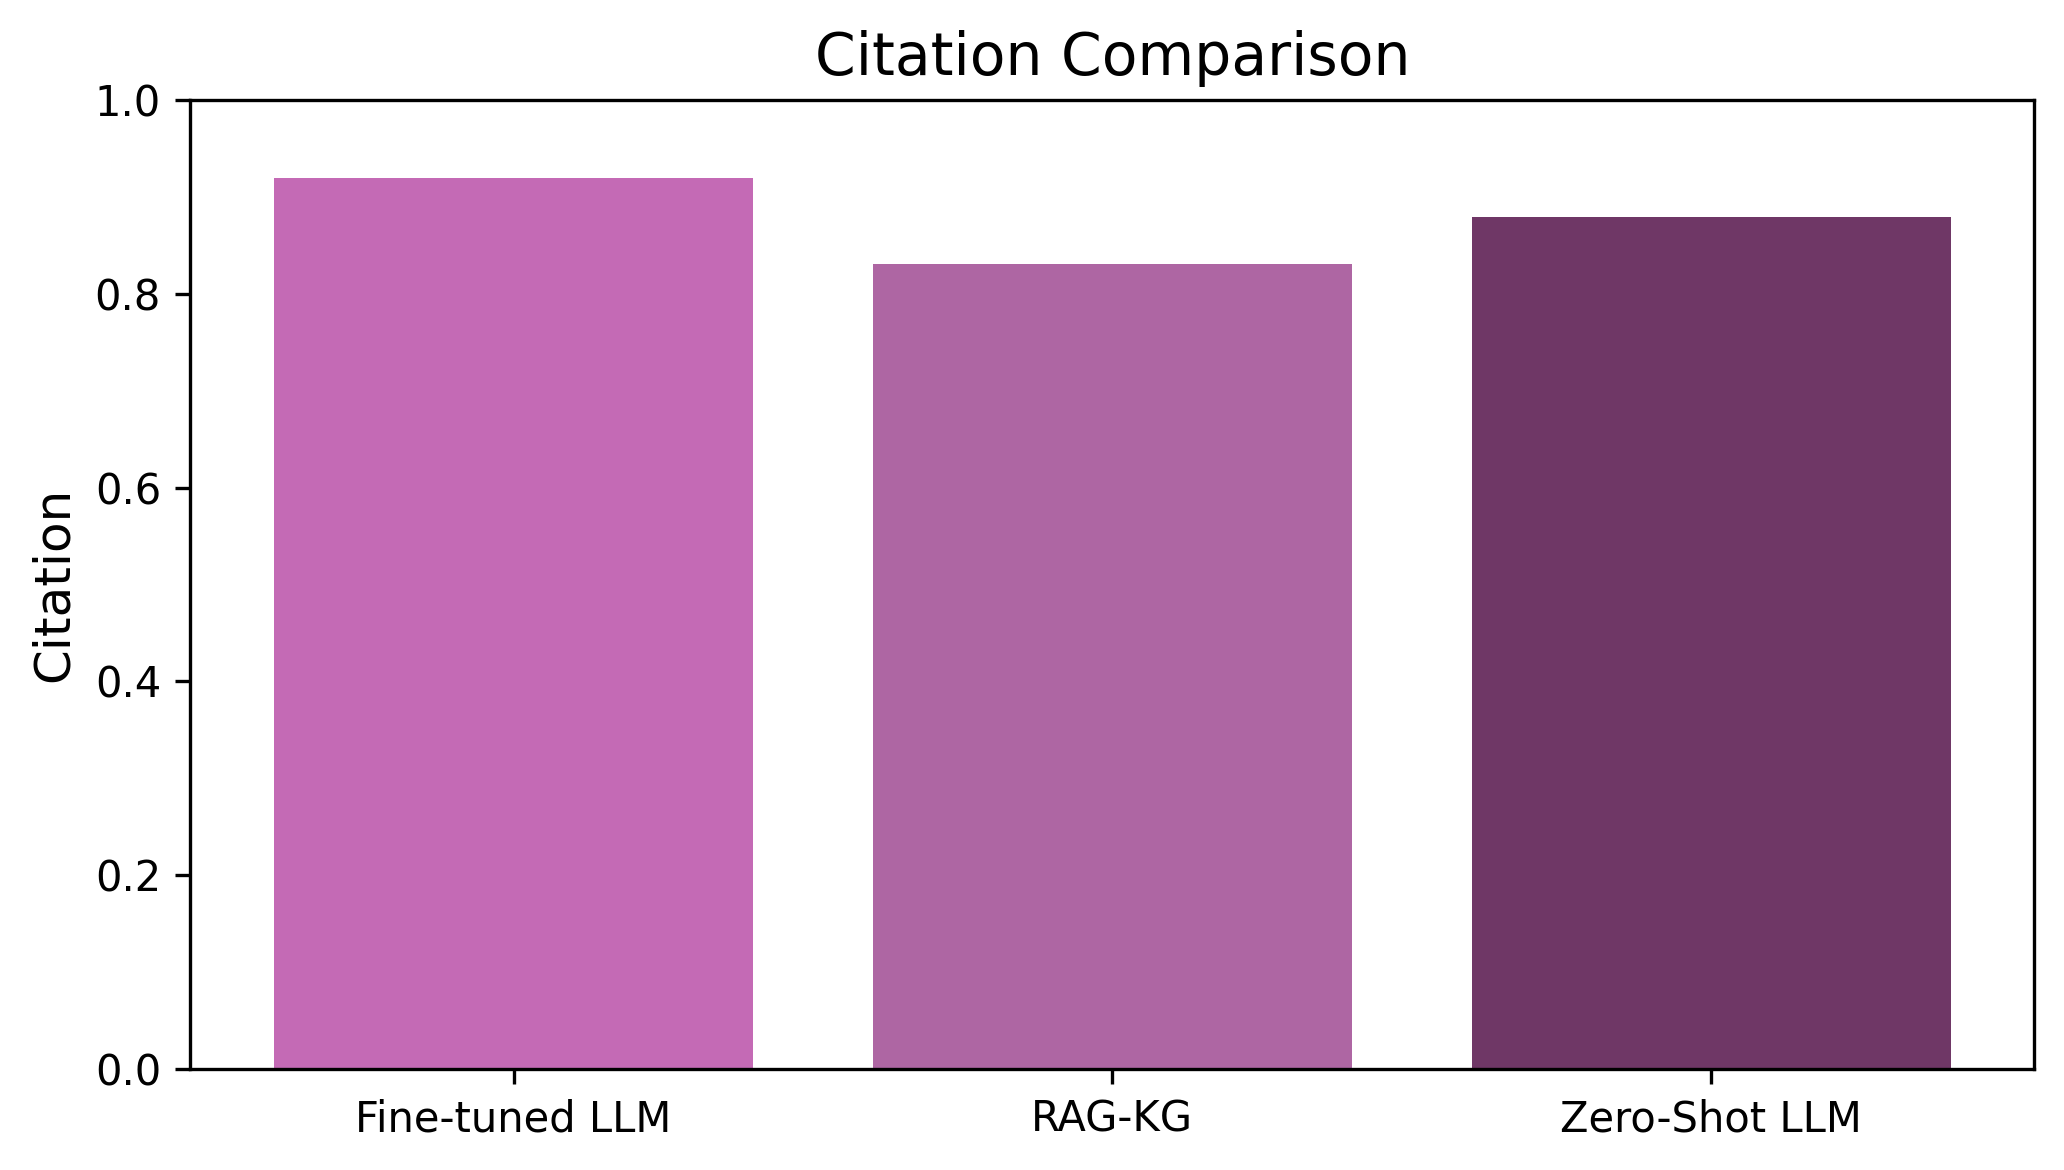
\includegraphics[width=\columnwidth]{images/eval/groq_comparison_citation_2.png}
    \caption{Citation correctness on three comparison models.}
    \label{fig:citation}
\end{figure}


\subsection{Hallucination detection and mitigation}

In the hallucination detection and mitigation phase, the hallucination rate of each of the three models was evaluated. The hallucination rate refers to the frequency with which a model generates false, fabricated, or unsupported information while maintaining a tone of confidence. A hallucination occurs when a model produces output that is factually incorrect, not grounded in input data or inconsistent with real-world knowledge.

\[
\text{Hallucination Rate} = \frac{\text{Number of hallucinated responses}}{\text{Total responses evaluated}}
\]

For this phase, hallucination detection focused exclusively on output content that could not be verified in the input data. For this purpose, subject–predicate–object triples were extracted from each generated response and checked against the knowledge graph. A response was classified as hallucinated if \textbf{at least one triple was not present in the knowledge graph}, indicating that the model introduced information not supported by the available evidence. The resulting value was converted into a percentage, producing the outcomes shown in Figure~\ref{fig:hallucination}. As illustrated, the fine-tuned LLM once again achieved the lowest hallucination rate, demonstrating the most reliable behavior among the three models.

\begin{figure}[h!]
    \centering
    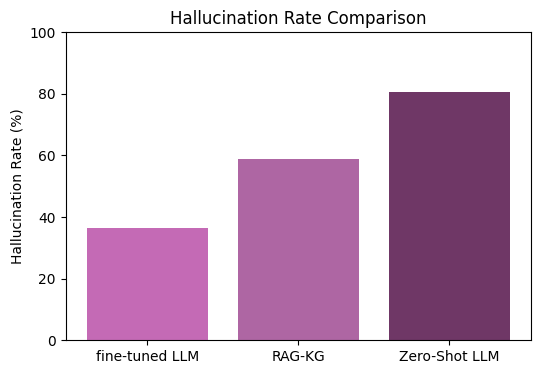
\includegraphics[width=\columnwidth]{images/eval/hallucination_rate_2.png}
    \caption{Hallucination rate \% on three comparison models.}
    \label{fig:hallucination}
\end{figure}

Finally, after inspecting the identified hallucinations, it was observed that for the zero-shot LLM, several instances were classified as hallucinations, although they represented factual relations that simply were not present in the PDF source and, consequently, not included in the knowledge graph. Therefore, the actual hallucination rates of Zero-shot baseline models would likely be lower than reported, although still higher than that of the fine-tuned LLM.

\subsection{Delivery and demo}

To illustrate the practical utility of the developed system, an interactive question–answering demo was implemented using the Gradio framework. The interface allows users to query the knowledge base in three operational modes: Zero-shot, RAG-KG, and Fine-tuned. User input is processed through backend functions that call the corresponding reasoning pipeline, returning both an answer and its grounding sources (page references from the original document).
This demo enables direct comparison between model modes and demonstrates how structured knowledge from our reference document can be transformed into interpretable grounded responses.

\begin{figure}[h!]
    \centering
    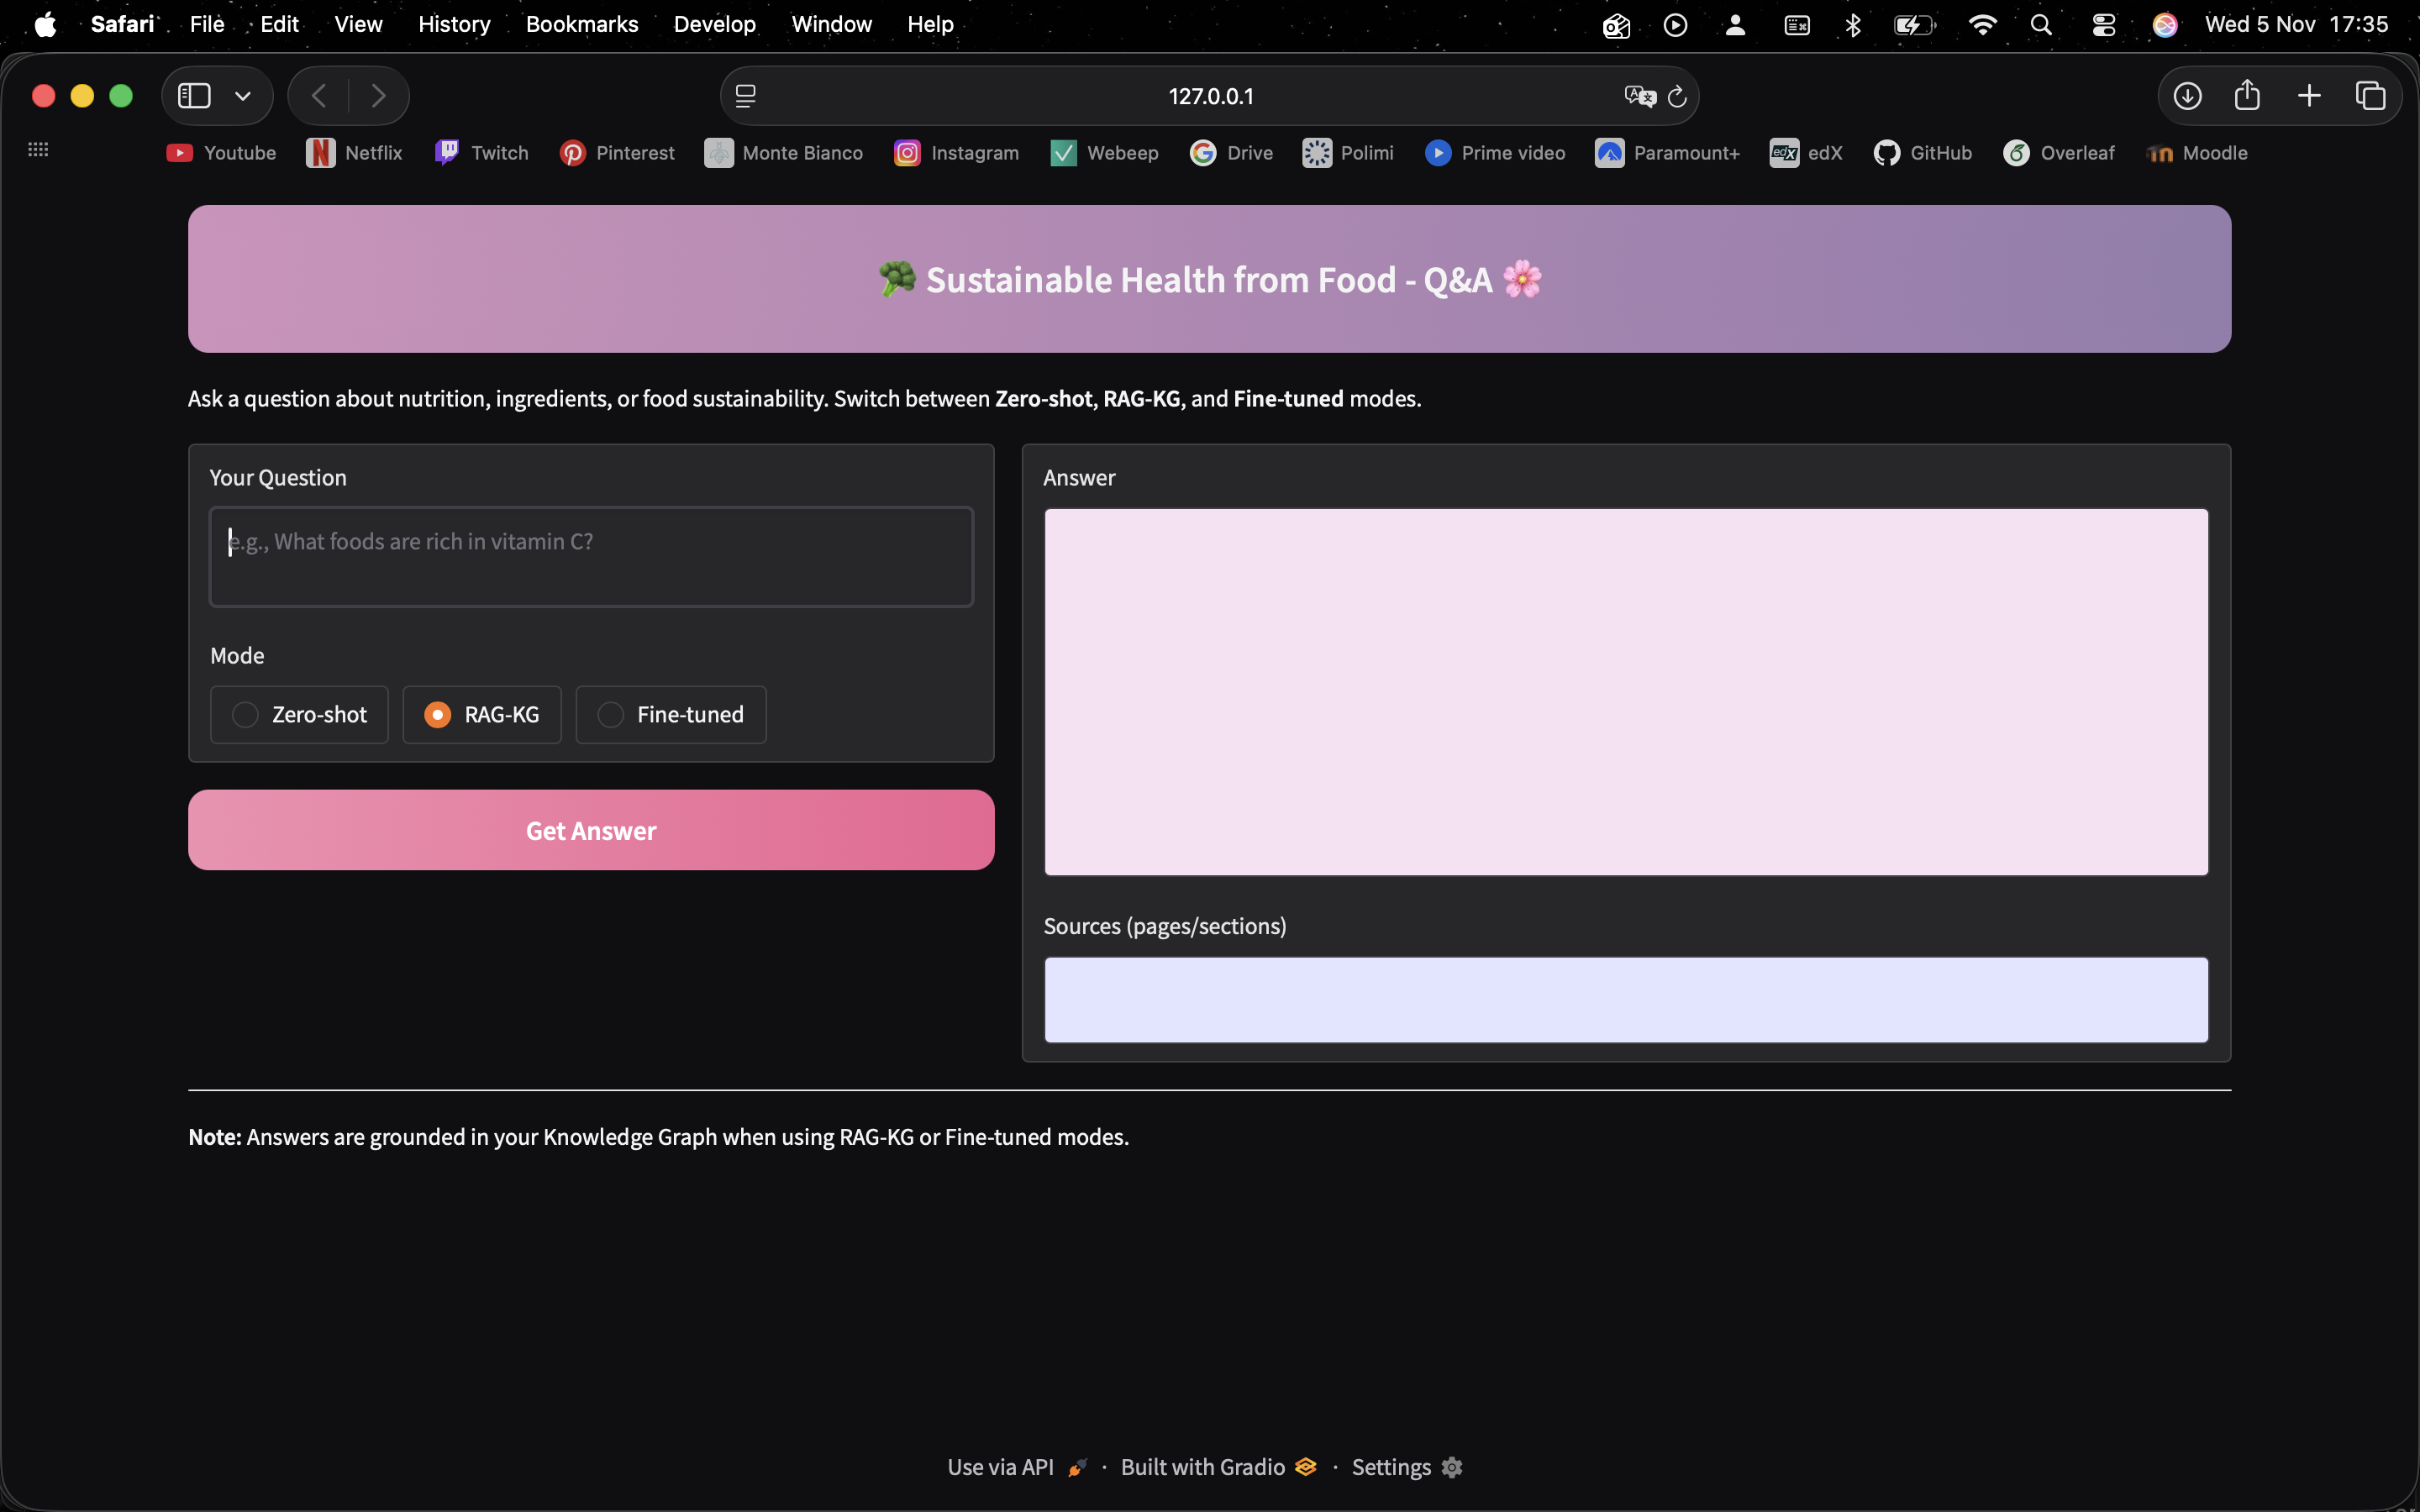
\includegraphics[width=\columnwidth]{images/gui_example/demo-plain.png}
    \caption{UI demo, initial window.}
    \label{fig:ui_demo_plain}
\end{figure}
\begin{figure}[h!]
    \centering
    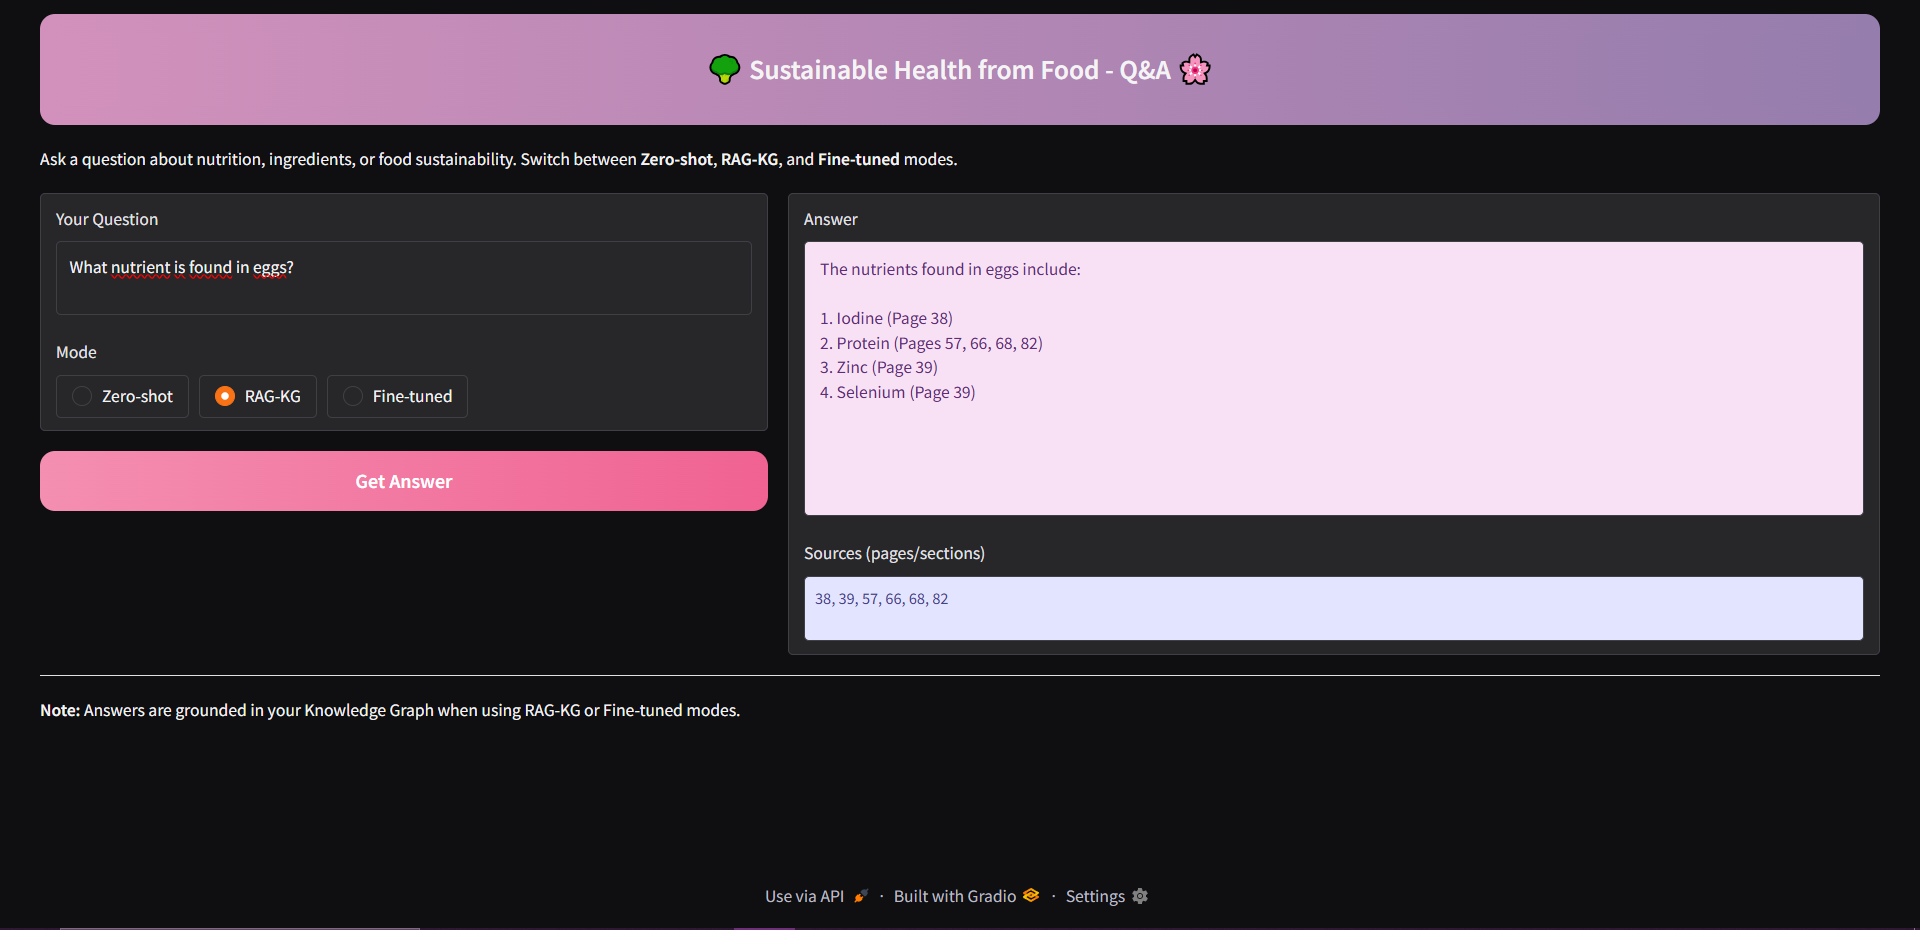
\includegraphics[width=\columnwidth]{images/gui_example/rag_kg_gui.png}
    \caption{Example of use of RAG-KG to answer question.}
    \label{fig:ui_demo_rag}
\end{figure}
\begin{figure}[h!]
    \centering
    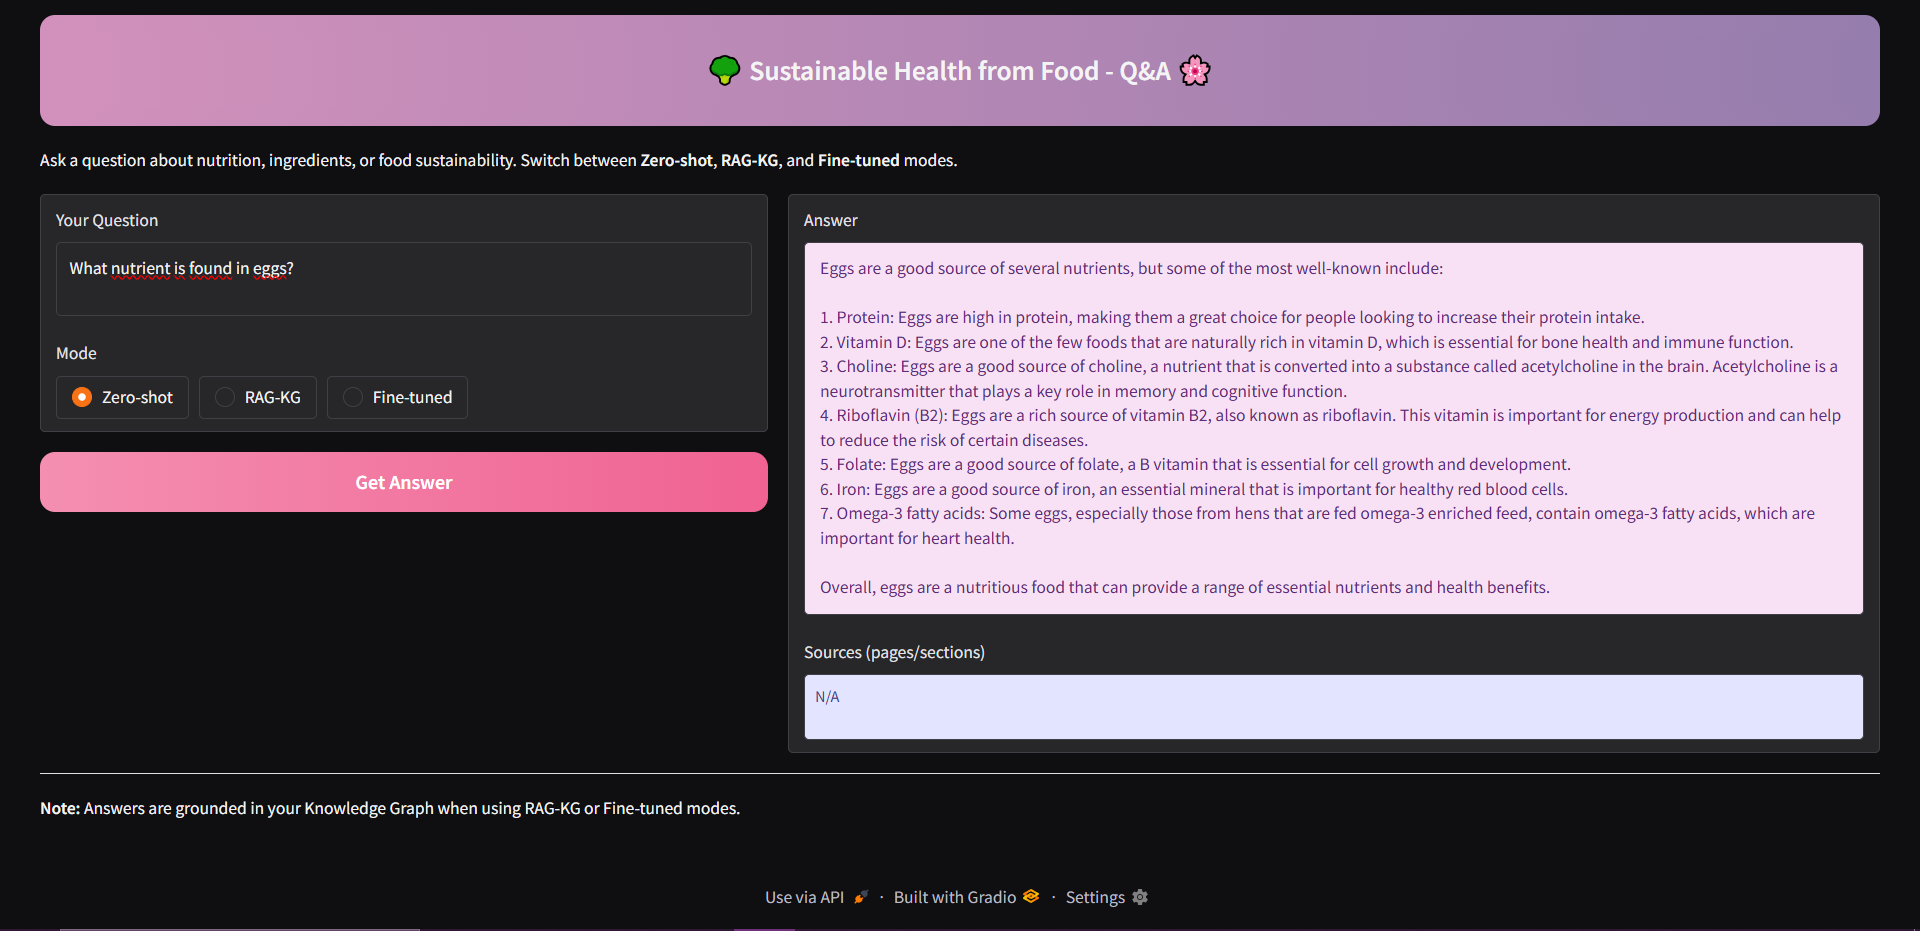
\includegraphics[width=\columnwidth]{images/gui_example/zero_shot_gui.png}
    \caption{Example of use of Zero-Shot to answer question.}
    \label{fig:ui_demo_zero}
\end{figure}
\begin{figure}[h!]
    \centering
    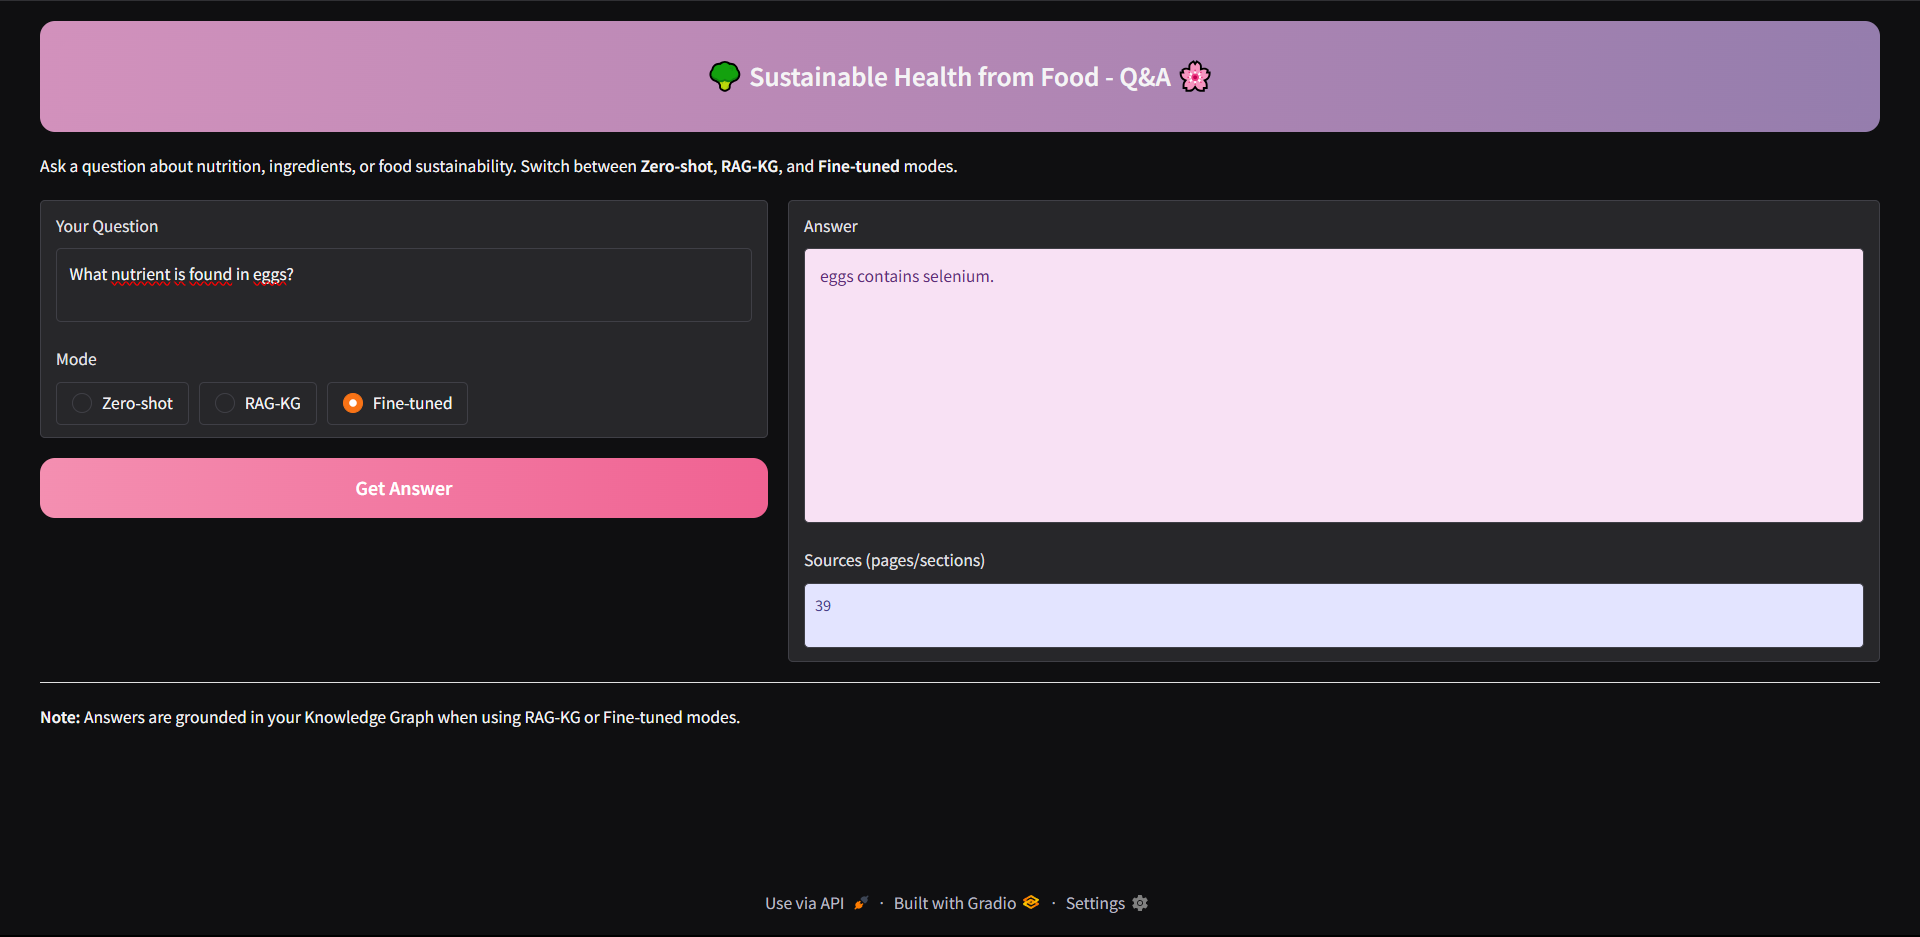
\includegraphics[width=\columnwidth]{images/gui_example/fine_tuned_gui.png}
    \caption{Example of use of our fine tuned model to answer question.}
    \label{fig:ui_demo_fine}
\end{figure}


\section{Results and Discussions}

The results of the project's pipeline are analysed at multiple levels: the quality of the extracted and structured knowledge resulting from PDF parsing and KG construction, the characteristics of the grounded generation of the instruction-response dataset, the behaviour of large language models using different setups and finally the reliability of the generated answers. 

From a knowledge representation perspective, the extracted knowledge graph captures the key entities and relations that appear in the original source document. This enables the models used further on in the pipeline to create meaningful connections between food items, nutrients, dietary guidelines and health outcomes, to finally allow the execution of structured queries that would have been otherwise not possible if only considering the original PDF document. An advantage of how the knowledge construction was performed is that section-level and page-level metadata were saved to further support traceability later on in the process. However, the overall quality of the extracted knowledge highly depends on the rule-based and sentence-level nature of the extraction process, which might overlook implicit or long-range relations in the text\cite{relationextraction}. In particular, the method used for generating triples exclusively relies on domain-informed relation rules and only finds relations among entities that appear in the same section and the same sentence. This is optimal in most cases, but might skip certain relations that do not follow that exact structure. This limitation might affect the overall pipeline, as missing or simplified relations could directly influence the scope of the generated instruction–response dataset and the subsequent evaluation of grounded model outputs.

Regarding the grounded dataset creation, the automatically generated instruction–response dataset clearly reflects the structure and coverage of the underlying knowledge graph. By transforming the previously obtained triples into natural language questions and answers, the resulting dataset contains instructions that are all grounded in explicit relations extracted from the source document. Advantages of the employed method for instruction-response generation include the diversification of question types (factoid, list-based, reasoning and constraint-oriented) to ensure good coverage of possible real-life cases as well as the inclusion of page-level citations for each response to enhance transparency and allow verification on the original report. However, because the dataset is derived exclusively from the constructed knowledge graph, its scope is inherently limited to the relations explicitly captured during extraction, as mentioned before. This results in a tendency toward concise and structurally homogeneous answers, which influences both the fine-tuning process and the evaluation setup performed after this step.

At the model level, clear behavioural differences emerged between the fine-tuned language model, the retrieval-augmented (RAG-KG) setup, and the zero-shot baseline when applied to the same set of grounded instructions. The fine-tuned model consistently produced concise and well-structured answers that closely followed the format of the instruction–response dataset, including explicit citations to the source document. This behaviour reflected its exposure to the grounded training data and resulted in high scores on automatic metrics, particularly those sensitive to lexical overlap and formatting consistency. In contrast, the zero-shot model tended to generate more verbose and explanatory responses, often incorporating additional background information that is not explicitly present in the source document. While this could improve perceived completeness, it also increased the likelihood of ungrounded statements, as explained in section \ref{subsec:eval}. The RAG-KG setup exhibited an intermediate behaviour: its responses were constrained by the retrieved triples and therefore more grounded than zero-shot outputs, but they remained sensitive to retrieval quality and might exclude relevant information when the matching process failed. Overall, these observations indicated that different grounding strategies lead to distinct trade-offs between answer conciseness, completeness, and factual alignment with the extracted knowledge. A summary of the performance comparison between the three different setups can be seen in table \ref{tab:model_comparison}, while the complete evaluation of the models was previously explained in section \ref{subsec:eval}: \textit{Evaluation}.


\begin{table*}[t]
\centering
\caption{Performance comparison across different model setups}
\label{tab:model_comparison}
\resizebox{\textwidth}{!}{%
\begin{tabular}{lccccccccccccc}
\hline
\textbf{Model} &
\textbf{F1} &
\textbf{ROUGE-1} &
\textbf{ROUGE-2} &
\textbf{ROUGE-L} &
\textbf{BLEU-1} &
\textbf{BLEU-2} &
\textbf{BLEU-3} &
\textbf{BLEU-4} &
\textbf{CSR} &
\textbf{Rel.} &
\textbf{Comp.} &
\textbf{Cit. Corr.} &
\textbf{Hall. Rate} \\
\hline
Zero-shot LLM   & 0.08 & 0.07 & 0.02 & 0.09 & 0.06 & 0.02 & 0.02 & 0.02 & 0.91 & \textbf{0.84} & \textbf{0.85} & 0.87 & 80.90\% \\
RAG-KG          & 0.10 & 0.11 & 0.05 & 0.11 & 0.07 & 0.04 & 0.03 & 0.02 & \textbf{1.00} & 0.62 & 0.56 & 0.82 & 59.80\% \\
Fine-tuned LLM  & \textbf{0.69} & \textbf{0.71} & \textbf{0.53} & \textbf{0.70} & \textbf{0.68} & \textbf{0.58} & \textbf{0.47} & \textbf{0.41} & 0.55 & 0.68 & 0.47 & \textbf{0.92} & \textbf{37.30\%} \\
\hline
\end{tabular}%
}
\end{table*}








With respect to the reliability of the generated answers, clear differences emerged across the three evaluated model setups. The fine-tuned model consistently demonstrated the highest level of factual alignment with the extracted knowledge, as reflected by its low hallucination rate. This behaviour can be attributed to its training on grounded instruction–response pairs that explicitly linked each answer to source-level evidence. In contrast, the zero-shot model exhibited a higher incidence of hallucinated content, primarily due to its tendency to draw on general background knowledge that is not explicitly supported by the source document. While some of these responses might be factually correct in a broader sense, they remained ungrounded with respect to the constructed knowledge graph and are therefore classified as hallucinations under the adopted evaluation criteria. The RAG-KG setup was again in an intermediate position: its reliance on retrieved triples constrained generation to supported facts when retrieval succeeded, but incomplete or imprecise retrieval could still result in omissions or unsupported statements. Overall, these findings highlighted the role of explicit grounding and structured knowledge in improving the reliability and traceability of language model outputs, particularly in domain-specific settings like the one analysed. 
\section{Overall Discussions}

The integrated pipeline demonstrated how structured knowledge extraction and large language model reasoning can be combined in a reproducible and interpretable framework. By connecting ontology-driven semantic structures to downstream generative tasks, the system bridged symbolic knowledge representation and data-driven natural language understanding. This approach enabled not only accurate information retrieval but also transparent and traceable reasoning, as every model output can be linked back to its source document.

A limitation encountered was that, after an extensive search for papers related to our analysis, no comparable studies were found, likely due to the specificity of the topic and the architecture implemented. 

Overall, the results demonstrated how design choices at each stage of the pipeline directly influenced the behaviour and reliability of language model outputs. Both benefits and constraints of grounding generative models in structured knowledge were highlighted, emphasizing the trade-offs between factual alignment, completeness, and generality.
\section{Conclusion}

In recent years, the combination of structured knowledge representation and large language models has opened new opportunities for building systems that are both intelligent and interpretable. Ontologies and knowledge graphs play a crucial role in this space, providing the foundation for organizing complex domain knowledge in a transparent and reusable way. When integrated with generative models, they enable a new form of reasoning, one that combines the precision of structured data with the flexibility of natural language understanding.
In domains such as food, nutrition, and sustainability, this integration is particularly important. These areas require not only factual accuracy, but also contextual understanding, scientific traceability, and sensitivity to public health and environmental concerns. Structuring information about ingredients, nutrients, and health outcomes in a formal schema allows knowledge to be shared, queried, and validated across systems, supporting more consistent and evidence-based communication.
More broadly, this direction illustrates a shift toward AI systems that are not just powerful, but explainable and accountable. By grounding model outputs in well-defined knowledge structures, we move closer to applications that support education, policy, and decision-making in transparent and trustworthy ways.

% References
\bibliographystyle{IEEEtran}
\bibliography{references/references}



% Appendix
%\appendix
%\section*{Appendix}

\end{document}
